\documentclass{ntnuthesis}

\usepackage{amsmath}
\usepackage{amsthm}

\usepackage[sf]{titlesec}				% Title options	
\usepackage{calc}						% \setcounter{ctr}{num} tools
\usepackage{pdfpages}					% \includepdf tools	
%\usepackage{cleveref}					% \cref{} tools
\usepackage{booktabs}					% Table options
\usepackage{afterpage}					% Upgrade on \clearpage
%\usepackage{showframe}
%\usepackage[nottoc,notlot,notlof]{tocbibind}
	
\usepackage[slantedGreek,sc]{mathpazo}	% Font options
\usepackage{avant}						% Font options
\usepackage{microtype}					% Font options
\usepackage[greek,english]{babel}		% Typographical rules (?)

\usepackage{pagecolor,xcolor}
\usepackage{graphicx}
\usepackage{caption}
\usepackage[caption=false]{subfig}
\usepackage{adjustbox}



\usepackage[avantgarde]{quotchap}

%% BIBLIOGRAPHY OPTIONS ============================================

\usepackage[  
backend     = bibtex, % biber or bibtex
doi         = false,
url         = true,
isbn        = false,
labeldate   = true,
eprint      = true,
maxbibnames = 99,
natbib      = true,
sorting     = nyt,
style       = numeric,
defernumbers= true
]{biblatex}












%\renewbibmacro{in:}{\ifentrytype{article}{}{\printtext{\bibstring{in}\intitlepunct}}}

%\AtEveryBibitem{
%  \clearfield{abstract}
%}

%
%\addbibresource{references}
%\addbibresource{referencesBooks}
%\addbibresource{referencesSoftwares}
\addbibresource{D:/OneDrive_NTNU/SWwd/LaTEX/ADWELL}

%% PACKAGES TURNED OFF =============================================

%\usepackage[utf8]{inputenc}
%\usepackage[T1]{fontenc}
\usepackage{verbatim}		% commenting environment

\usepackage{url}
\usepackage{todonotes}


% This after {cleverref} produces hyperlinks on \ref{} and \eqref{}
%\usepackage[pdfborder={0 0 0},hyperfigures]{hyperref}

%\floatsetup{ 
%  heightadjust=object,
%  valign=t
%}










%% ALEX =============================================


\usepackage{etoolbox}

% Nomenclature
\usepackage[intoc]{nomencl}
\makenomenclature
% Documentation: http://texdoc.net/texmf-dist/doc/latex/nomencl/nomencl.pdf


\usepackage{fancyhdr}

\usepackage{biblatex}


\usepackage[ %
pdfproducer={Texmaker},     % 
pdfcreator={pdfLaTeX},      % 
hidelinks,                  % versteckt die Boxen um die Links in der PDF
bookmarksnumbered,          % nummereiert Lesezeichen
]{hyperref}     




\usepackage{cleveref}					% \cref{} tools



% NEW MATH COMMANDS ================================================
\setlength\emergencystretch{\hsize}
\newcommand{\diff}{\mathrm{d}}

\def\SL{S_{\mathrm{L}}}
\def\SR{S_{\mathrm{R}}}
\def\SC{S_{\mathrm{C}}}
\def\CL{c_{\textup{L}}}
\def\CR{c_{\textup{R}}}

\def\SLj{S_{\mathrm{L},j+1/2}}
\def\SRj{S_{\mathrm{R},j+1/2}}

\def\ASj{A_{\mathrm{S},j+1/2}}
\def\QSj{Q_{\mathrm{S},j+1/2}}

\def\ul{u_{\textup{L}}}
\def\ur{u_{\textup{R}}}

\newtheorem{theorem}{Theorem}
\newtheorem{definition}{Definition}
\newtheorem{lemma}{Lemma}
\newtheorem{proposition}{Proposition}
\newtheorem{remark}{Remark}
\newcommand{\betag}{\greektext b\latintext}
\allowdisplaybreaks

%% TITLEPAGE ENVIRONMENT FOR THE PAPERS ============================

\newenvironment{journalpaper}[1]
	{\begin{titlepage}
		\newpagecolor{cyan!15}
		\centering
		{\sffamily\large\bfseries Journal paper #1} \\ [1cm]
		\rule{\linewidth}{0.5mm}
		}{
		\rule{\linewidth}{0.5mm}
	\end{titlepage}
%	\cleardoublepage
	\restorepagecolor
	\newpagecolor{white}
	}

\newenvironment{conferencepaper}[1]
	{\begin{titlepage}
	\newpagecolor{cyan!15}
	\centering
	{\sffamily\large\bfseries Conference paper #1} \\ [1cm]
	\rule{\linewidth}{0.5mm}
    }{
    \rule{\linewidth}{0.5mm}
  \end{titlepage}
%  \cleardoublepage
  \restorepagecolor
  \newpagecolor{white}
}

%% TITLE AND .PDF FILE INFORMATION =================================

%% Set PDF file information
%\hypersetup{
%pdfinfo={
%	Title={Large Time Step Methods for Hyperbolic Conservation Laws},
%	Author={Marin Prebeg},
%	Subject={PhD thesis},
%}}

\title{Turbulence structure and particle transport\\in particle loaded non-Newtonian Fluids}
\author{Alexander Busch}
\degreetype{Philosophiae doctor}
\faculty{Faculty of Engineering}
\department{Department of Energy and Process Engineering}
\isbnprinted{978-82-326-2638-0}
\isbnelectronic{978-82-326-2639-7}
\serialnumber{2019:285}

\begin{document}
%\fuzzy
%\sloppy

\pagestyle{empty}
% Includes page number at the bottom of the page.
\maketitle

% Marin
%\pagestyle{plain}
% Includes page number at the bottom of the page.
\pagenumbering{roman} 				
% Uses small roman numbers for page numbering.
\setcounter{page}{3}
% Resets the page counter to 1.


% Headers and Footers (https://tex.stackexchange.com/questions/151784/how-to-display-current-section-title-in-header)
\pagestyle{fancy}
\fancyhf{}
%\fancyhead[LE]{\nouppercase\leftmark}
\fancyhead[LE]{\bfseries\nouppercase{\ifnum\value{chapter}>0 \thechapter\ \fi\leftmark}}
\fancyhead[RO]{\nouppercase\rightmark}
\renewcommand{\headrulewidth}{0pt}
\renewcommand{\chaptermark}[1]{\markboth{#1}{}}
\setlength{\headheight}{14.5pt} % very important!
\fancyfoot[LE,RO]{\thepage}
%\fancyfootoffset[le,ro]{30pt}


\chapter*{Abstract}
\addcontentsline{toc}{chapter}{Abstract}
\input{Content/01_Abstract}
\clearpage
\shipout\null

\chapter*{Preface}
\addcontentsline{toc}{chapter}{Preface}

The work presented in this thesis was carried out in the period from September 2014 to July 2017, at the Department of Energy and Process Engineering at the Norwegian University of Science and Technology. The project has been funded through the SIMCOFLOW project, carried out by the SINTEF Materials and Chemistry. I gratefully acknowledge the financial support from the Research Council of Norway (project no.~234126/30). 

I wish to thank my supervisor, Professor Bernhard M\"{u}ller, for allowing and encouraging me to pursue my own ideas, while ensuring that I stay on planned schedule and agreed deadlines. I am especially thankful for a lot of patience during the beginning of my PhD when I had a lot to learn and catch up with. I would like to thank my co-supervisor Tore Fl{\aa}tten for all our scientific and nonscientific discussions. I am especially thankful for teaching me countless mathematical concepts and tools and for having endless faith in our work even when I didn't. I wish to thank my co-supervisor Marica Pelanti for arranging my stay at ENSTA ParisTech and for being a great host during my six months stay in Paris. My stay in Paris has been a valuable experience both professionally and personally. Further, Marica's knowledge on HLL(C) schemes has been an invaluable asset when I first started to work with this schemes. I also wish to thank my co-supervisor Ernst Arne Meese. We did not collaborate closely, but I appreciated our discussions and interest in my work.

These three years would have been much less fun without all my co-workers from the Department of Energy and Process Engineering. I am very thankful for all Green Room breaks, movie nights, dinners and skiing trips, but most of all, thank you for sharing with me the joys and excitement of doing sweet science. There are too many people to name them all, and I will point out {\O}yvind, Ehsan, Eskil and Anna who had a misfortune of sharing an office and an apartment with me. 

Lastly, I wish to thank all my friends back home in German for not forgetting me during my long absences, and I wish to thank Martina for her endless support in all my endeavors. 

\vspace*{2\baselineskip}

\hfill Trondheim, December 2018

\hfill Alexander Busch

\clearpage
\shipout\null

\chapter*{Acknowledgments}
\addcontentsline{toc}{chapter}{Acknowledgments}
\input{Content/03_Acknowledgments}
\clearpage
\shipout\null

%\chapter*{Nomenclature}
%\addcontentsline{toc}{chapter}{Nomenclature}
\printnomenclature
\clearpage
\shipout\null
% Execute "makeindex thesis.nlo -s nomencl.ist -o thesis.nls" in thesis path to generate .nls file and recompile
% Documentation: http://texdoc.net/texmf-dist/doc/latex/nomencl/nomencl.pdf


\tableofcontents				
\addcontentsline{toc}{chapter}{Contents}
\clearpage


% Uses small roman numbers for page numbering.
\pagenumbering{arabic} 				
% Resets the page counter to 1.
\setcounter{page}{1}

\chapter{Introduction}
\label{cha:Introduction}

\section{Motivation}

phenomena \cite{busch2018}
phenomena~\cite{busch2018a}
phenomena~\cite{busch2018b}
phenomena~\cite{busch2018c}
phenomena~\cite{busch2017}\\

phenomena~\cite{aarsnes2018}
phenomena~\cite{khatibi2017}
phenomena~\cite{busch2017a}
phenomena~\cite{busch2016}
phenomena~\cite{zoric2015}\\

\nomenclature{$x$}{Description}
\nomenclature{$y$}{Description}

Hyperbolic conservation laws are widely used to model a variety of physical phenomena, such as fluid dynamics, geophysics, biomechanics, electrodynamics, magnetohydrodynamics, astrophysics, etc. They are also heavily used in modeling multiphase flow phenomena~\cite{doraiswamy2002}, which is of particular interest for the SIMCOFLOW project~\cite{wallis1969}\footnote{The PhD project is a part of the research project \textit{SIMCOFLOW -- a framework for complex 3D multiphase and multi physics flows} carried out by SINTEF Materials and Chemistry from July 2014 until June 2017 and funded by the Research Council of Norway.}. In this thesis, we consider already existing models and focus on numerical methods for hyperbolic conservation laws rather than on physical modeling. To simplify the analysis, we mostly use simpler models (such as the Euler equations) instead of more complicated multiphase flow models. However, we believe that the numerical tools developed here should be applicable to a wide class of hyperbolic problems.

\section{State of the art}
\label{sec:history}


\section{Goals and thesis outline}
\label{cha1:sec:goals}

 In particular, our goals are:
\begin{itemize}
\item Develop LTS extensions of the HLL and HLLC schemes.
\item Study entropy stability of the LTS-HLL(C) schemes.
\item Study positivity preservation of the LTS-HLL(C) schemes.
\item Study boundary and source term treatment in the LTS methods.
\end{itemize}

The thesis outline and contributions can be summarized as follows: in chapter~\ref{cha:Background} we present the mathematical models we solve, we outline the framework of the numerical methods we will consider, and we present the existing LTS methods. In chapter~\ref{cha:LTS-HLL} we present the main results:
\begin{itemize}
\item In \cref{sec:LTS-HLL(C)} we develop LTS extensions of the HLL and HLLC schemes. We develop the LTS-HLL-type schemes, we determine their numerical viscosity and flux-difference splitting coefficients, and we investigate their convergence. This new class of schemes allows us to deduce some already existing LTS methods such as the LTS-Roe and LTS-Lax-Friedrichs, and it allows us to deduce LTS extensions of other methods, such as the Rusanov and Engquist-Osher schemes. Parts of this section are adapted from our second journal paper \textit{Large Time Step HLL and HLLC Schemes}~\cite{jp2}.

\item In \cref{sec:EV-ME} we study entropy stability of LTS-HLL-type schemes. We use modified equation analysis to investigate how entropy violations occur in the LTS-HLL-type schemes and how can they be avoided. Parts of this section are adapted from our second conference paper \textit{Numerical Viscosity in Large Time Step HLL-type Schemes}~\cite{cp2}.

\item In \cref{sec:PP} we study monotonicity and positivity preservation of LTS-HLL(C) schemes. We determine monotonicity conditions on numerical flux function of an LTS method, and we show that positivity preserving conditions in LTS methods are stronger than in standard methods. We investigate different ways how is positivity lost in the LTS-HLL scheme, and we propose a simple way to increase robustness of the scheme by adding numerical diffusion. This section closely follows our third journal paper \textit{Monotonicity and Positivity Preservation in Large Time Step Methods}~\cite{jp3}.
\end{itemize}

In addition to the work on the LTS-HLL(C) schemes, we applied the LTS-Roe scheme to a one-dimensional two-fluid model and focused on the treatment of the source terms and the boundary conditions. By introducing a new type of boundary conditions and by treating source terms in a similar way as 


, we are able to notably improve accuracy of the solution. These results are presented in~\cref{cha:MPM}. Content of \cref{cha:MPM} corresponds to our first journal paper \textit{Large Time Step Roe Scheme for a Common 1D Two-Fluid Model}~\cite{jp1}, and our first conference paper \textit{Boundary and Source Term Treatment in the Large Time Step Method for a Common Two-Fluid Model}~\cite{cp1}. Finally, \cref{cha:Conclusions} closes with conclusions and comments regarding possible further research directions.

In the presentation of the thesis results, we aimed to give a structured overview of our findings, but also tried to depict the order in which our work was done and how it was motivated.


\clearpage

%
\begin{savequote}[50mm]
Never any knowledge was delivered in the same order it was invented.
%\footnotemark[1]
\qauthor{Sir Francis Bacon}
\end{savequote}

\chapter{Background}
\label{cha:Background}

%\footnotetext[1]{In \textit{Valerius Terminus: Of the Interpretation of Nature}, c. 1603.}
%\setcounter{footnote}{1}

We present the mathematical models we will be considering and the numerical methods we will be using. 

First, we present a general scalar conservation law and the Euler equations. The multiphase flow model will be presented in \cref{cha:MPM}. The properties of the solution to the scalar conservation law are presented in more detail, with a focus on the uniqueness of the solution and entropy conditions.

We then present the numerical methods we will use. We begin with the standard methods for scalar conservation laws and consider their numerical viscosity and flux-difference splitting forms. Convergence and entropy stability of the numerical methods are discussed following the standard literature. We do not aim to provide a comprehensive overview of numerical methods for the hyperbolic conservation laws. Instead, we focus on those parts that play an important role in the understanding and development of LTS methods. The methods are then extended to the LTS framework along the lines of Lindqvist et al.~\cite{lin16}. Main ideas of the LTS methods are presented, together with the already existing LTS methods. 

Finally, both standard and LTS methods are extended to systems of conservation laws following the standard field-by-field decomposition.

The content of this chapter up to \cref{sec:Background:scalar-LTS-methods} on the LTS methods heavily builds on the existing literature, and we refer to the books by Godlewski and Raviart~\cite{god96}, LeVeque~\cite{lev92,lev02}, Toro~\cite{tor09}, Trangenstein~\cite{tra09} and Dafermos~\cite{daf10} for more detailed reading.

\section{Mathematical models}

\subsection{Scalar conservation laws}
\label{sec:SCL}

We consider the initial value problem for the scalar conservation law:
\begin{subequations} \label{eq:SCL}
\begin{align}
u_t + f(u)_x & = 0, \qquad x \in \mathbb{R}, \, t \in \mathbb{R}^+, \label{eq:SCL-a} \\
u(x,0) & = u_0(x), 
\end{align}
\end{subequations}
where $ u \in \mathbb{R} $ is a conserved variable, $ f(u): \mathbb{R} \rightarrow \mathbb{R} $ is a strictly convex (or concave) flux function\footnote{Here and throughout the thesis, we will be considering only strictly convex (i.e. \mbox{$ f''(u) > 0 $}) or strictly concave (i.e. $ f''(u) < 0 $) flux functions.}, and $ u_0 $ is the initial data.\footnote{We follow the common notation where subscripts $ x $ and $ t $ denote partial derivatives with respect to $ x $ and $ t $, respectively.} It is known that solutions to the initial value problem \eqref{eq:SCL} may develop discontinuous solutions even when the initial data is smooth. To allow for discontinuous solutions we consider weak solutions that satisfy \eqref{eq:SCL} in the sense of distributions. A function $ u(x,t) $ is a weak solution of \eqref{eq:SCL} if it satisfies:
\begin{equation} \label{eq:weak-form}
\int_{0}^{\infty} \int_{-\infty}^{+\infty} \left( u \varphi_t + f(u) \varphi_x \right) \diff x \diff t + \int_{-\infty}^{+\infty} u_0(x) \varphi(x,0) \diff x = 0,
\end{equation}
for all test functions $ \varphi \in C_0^1 $, i.e. for all continuously differentiable functions with compact support. However, there are infinitely many weak solutions $ u(x,t) $ that satisfy \eqref{eq:SCL} in a weak sense. The correct, unique weak solution to \eqref{eq:SCL} is the same as the solution to the parabolic equation:
\begin{equation} \label{eq:SCL-viscous}
u_t + f(u)_x = \nu u_{xx}, \quad \nu > 0,
\end{equation}
in the limit when $ \nu \rightarrow 0 $, where $ \nu $ is a small parameter acting as a viscosity. In order to determine if a particular weak solution $ u(x,t) $ is the unique weak solution, we usually determine the so-called \textit{entropy condition} for \eqref{eq:SCL} and check if the weak solution $ u(x,t) $ satisfies this condition. This can be done in different ways, and examples of such conditions include the Lax entropy condition~\cite{lax72}, Oleinik's entropy condition~\cite{ole57}, Kru\v{z}kov entropies~\cite{kru70} and entropy functions~\cite{lax72}. Here, we focus on the entropy functions, because they will be used later when we discuss the numerical methods.

The basic idea is to define an \textit{entropy function} $ \eta(u) $ such that it is a convex function of $ u $ (i.e. $ \eta''(u) > 0 $) and a corresponding \textit{entropy flux} $ \psi(u) $ such that:
\begin{equation}
\psi'(u) = \eta'(u) f'(u).
\end{equation}
Then it can be shown that the function $ u(x,t) $ is the unique weak solution (or \textit{entropy solution}) of the scalar conservation law \eqref{eq:SCL} if the inequality:
\begin{equation} \label{eq:SCL-entropy-inequality}
\eta(u)_t + \psi(u)_x \leq 0,
\end{equation}
holds in a weak sense, see LeVeque~\cite[p.~39]{lev92}.

Another important property of the unique weak solution to \eqref{eq:SCL} is that it respects a strict \textit{maximum principle}. Namely, if:
\begin{equation}
m = \underset{x}{\min} \left( u_0(x) \right), \quad
M = \underset{x}{\max} \left( u_0(x) \right),
\end{equation}
then:
\begin{equation} \label{eq:PDE-maximum}
u(x,t) \in [m,M] \quad \forall \quad x,t.
\end{equation} 
This property will play an important role later on when we discuss monotone methods for scalar conservation laws and positivity preserving methods for systems of equations.

For our purposes, we assume that the unique weak solution is known and want to know whether the numerical method converges to this solution.

\subsubsection{The one-dimensional Riemann problem}

In order to gain additional insight into the properties of the solution to the scalar conservation law \eqref{eq:SCL}, we consider a Riemann problem for \eqref{eq:SCL}:
\begin{equation} \label{eq:scalar-RP}
u(x,0) = \left\{ \begin{array}{ll}
	\ul \quad & \text{for} \quad x<0, \\[0.25em]
	\ur \quad & \text{for} \quad x>0, \end{array} \right.
\end{equation}
which is simply the conservation law \eqref{eq:SCL} with a piecewise constant initial data with a single discontinuity. By assuming a strictly convex flux function $ f(u) $ the solution to the Riemann problem is either:
\begin{itemize}
\item a shock:
\begin{equation} \label{eq:scalar-shock}
u(x,t) = \left\{ \begin{array}{ll}
	\ul \quad & \text{for} \quad x<st, \\[0.25em]
	\ur \quad & \text{for} \quad x>st, \end{array} \right.
\end{equation}
where $ s (\ul,\ur) $ is the shock speed given by the Rankine--Hugoniot condition:
\begin{equation}
s = \frac{f(\ur) - f(\ul)}{\ur - \ul},
\end{equation}
\item or a rarefaction wave:
\begin{equation} \label{eq:scalar-rarefaction}
u(x,t) = \left\{ \begin{array}{lll}
	\ul \quad & \text{for} \quad x \leq f'(\ul)t, \\[0.25em]
	(v(x/t)) \quad & \text{for} \quad f'(\ul)t \leq x \leq f'(\ur)t, \\[0.25em]
	\ur \quad & \text{for} \quad x \geq f'(\ur)t, \end{array} \right.
\end{equation}
where:
\begin{equation}
f'\left( v(x/t) \right) = \frac{x}{t}.
\end{equation}
\end{itemize} 
The structure of the solution for the Riemann problem \eqref{eq:scalar-RP} is closely related to the fact that \eqref{eq:SCL} has infinitely many weak solutions. Namely, it is possible to construct weak solutions of \eqref{eq:SCL} with the initial data \eqref{eq:scalar-RP} that satisfy \eqref{eq:SCL} in a weak sense, but are not the solution to the viscous equation \eqref{eq:SCL-viscous} in the vanishing viscosity limit.

The same difficulty is observed with numerical methods. When we numerically solve \eqref{eq:SCL} with discrete initial data \eqref{eq:scalar-RP}, a numerical method may converge to weak solution of \eqref{eq:SCL} that is not the solution to the viscous equation \eqref{eq:SCL-viscous} in the vanishing viscosity limit. We will return to this later on when we consider entropy stability of numerical methods.

\subsection{Systems of conservation laws}

We consider the hyperbolic system of conservation laws:
\begin{subequations} \label{eq:HSCL}
\begin{align}
\mathbf{U}_t + \mathbf{F(U)}_x & = 0, \qquad x \in \mathbb{R}, \, t \in \mathbb{R}^+, \\
\mathbf{U}(x,0) & = \mathbf{U}_0(x),
\end{align}
\end{subequations}
where $ \mathbf{U} \in \mathbb{R}^N $ ($ 1<N \in \mathbb{N} $) is a vector of conserved variables, \mbox{$ \mathbf{F(U)}: \mathbb{R}^N \rightarrow \mathbb{R}^N $} is a flux function, and $ \mathbf{U}_0 $ is the initial data. We can also write \eqref{eq:HSCL} in a quasilinear form as:
\begin{equation} \label{eq:QL}
\mathbf{U}_t + \mathbf{A(U)} \mathbf{U}_x = 0,
\end{equation}
where:
\begin{equation} \label{eq:Jacobian}
\mathbf{A(U)} = \frac{\partial \mathbf{F(U)}}{\partial \mathbf{U}},
\end{equation}
is the Jacobian matrix of $ \mathbf{F(U)} $. We assume that the system of equations \eqref{eq:QL} is hyperbolic, i.e. the Jacobian matrix \eqref{eq:Jacobian} has real eigenvalues and linearly independent eigenvectors.

Hyperbolic systems of conservation laws suffer from the same difficulties as the scalar conservation laws, i.e. they may develop discontinuous solutions and we have to look for a unique solution among all weak solutions. The unique entropy solution is determined in a similar fashion as for the scalar conservation law, namely we look for an entropy condition for the system of conservation laws and check if the particular weak solution satisfies this entropy condition. 

In general, the entropy conditions for systems of conservation laws are notably more difficult than for scalar conservation laws. For more details we refer to the literature from the beginning of this chapter and the work by Tadmor~\cite{tad86,tad87,tad03,tad16} and references therein. For our purposes, we will once again assume that the unique weak solution is known and we will only be interested in whether the numerical method converges to this solution.

\subsubsection*{The Euler equations}

The Euler equations can be written in the form \eqref{eq:HSCL} by defining:
\begin{equation} \label{eq:EE}
\mathbf{U} = \begin{bmatrix} \rho \\ \rho v \\ E \end{bmatrix},
\qquad
\mathbf{F(U)} = \begin{bmatrix} \rho v \\ \rho v^2 + p \\ v(E+p) \end{bmatrix},
\end{equation}
where $ \rho, v, E, p $ denote the density, velocity, total energy density and the pressure, respectively. The total energy density $ E $ is given as:
\begin{equation}
E = \rho e + \frac{1}{2} \rho v^2,
\end{equation}
where $ e $ is a specific internal energy defined by an equation of state:
\begin{equation}
e = e \left( \rho, p \right),
\end{equation}
which depends on the gas under consideration. In this thesis, we will consider only \textit{ideal gas} for which:
\begin{equation}
e = \frac{p}{\rho \left( \gamma - 1 \right)}.
\end{equation}
Throughout the thesis we will use $ \gamma = 1.4 $ for air. Alternatively, we may write the Euler equations \eqref{eq:EE} in the form \eqref{eq:QL} by defining the Jacobian matrix $ \mathbf{A(U)} $ (see LeVeque~\cite[p.~300]{lev02}). The eigenvalues of the Jacobian matrix $ \mathbf{A(U)} $ for the Euler equations are:
\begin{equation}
\lambda_1 = v - a, \quad \lambda_2 = v, \quad \lambda_3 = v + a,
\end{equation}
where $ a = \sqrt{\gamma p / \rho} $ is the speed of the sound. 
\begin{remark}
\textup{It is possible to define the Riemann problem \eqref{eq:scalar-RP} for the Euler equations and study structure of the solution in a similar fashion as for the scalar conservation law. We omit such analysis here and refer to Lax~\cite{lax72}, LeVeque~\cite{lev01} and Toro~\cite{tor09} for detailed analysis of the Riemann problem for the Euler equations.}
\end{remark}

\section{Finite volume methods for scalar conservation laws}
\label{sec:FVM-scalar}

We start by dividing the spatial domain into intervals with increment $ \Delta x = x_{j+1/2} - x_{j-1/2} $, and the time domain into intervals with increment $ \Delta t = t^{n+1} - t^n $. We then integrate the conservation law \eqref{eq:SCL} over the control volume $ \left[ x_{j-1/2}, x_{j+1/2} \right] \times \left[ t^n, t^{n+1} \right] $ to obtain:
\begin{align} \label{eq:scalar-integral}
\int_{x_{j-1/2}}^{x_{j+1/2}} u(x,t^{n+1}) \diff x & = \int_{x_{j-1/2}}^{x_{j+1/2}} u(x,t^n) \diff x \notag \\
 & \hspace{-7mm} + \int_{t^n}^{t^{n+1}} f(u(x_{j-1/2},t)) \diff t - \int_{t^n}^{t^{n+1}} f(u(x_{j+1/2},t)) \diff t,
\end{align}
which is telling us that the conserved variable inside a cell changes only due to the flow over its boundaries. By approximating the exact cell average of the exact solution as:
\begin{equation} \label{eq:CellAverage}
u_j^n \approx \frac{1}{\Delta x} \int_{x_{j-1/2}}^{x_{j+1/2}} u \left( x,t^n \right) \diff x,
\end{equation} 
and by approximating the time averaged flux function of the exact solution at the interface $ x_{j+1/2} $ as:
\begin{equation} \label{eq:FluxAverage}
F_{j+1/2}^n \approx \frac{1}{\Delta x} \int_{t^n}^{t^{n+1}} f(u(x_{j+1/2},t)) \diff t,
\end{equation}
we can write \eqref{eq:scalar-integral} in the conservation form:
\begin{equation} \label{eq:scalar-CF0}
u_j^{n+1} = u_j^n - \frac{\Delta t}{\Delta x} \left( F_{j+1/2}^n - F_{j-1/2}^n \right).
\end{equation}
%Unfortunately, it is in general not possible to evaluate the integral $ u\left( x_{j\mp 1/2,t} \right) $ exactly.
Unfortunately, $ u\left( x_{j\mp 1/2}, t \right) $ changes in time and most of the time we cannot evaluate the integral \eqref{eq:FluxAverage} exactly. Instead, we evaluate it by using an exact or approximate Riemann solver.

\subsection{Standard methods}
\label{s:standard-methods}

In order to solve \eqref{eq:SCL} numerically, Godunov~\cite{god59} assumes a piecewise constant initial data:
\begin{equation} \label{eq:piecewise-ID}
u(x,t^n) = u_j^n, \quad x_{j-1/2} \leq x < x_{j+1/2},
\end{equation}
which leads to a local Riemann problem defined at each interface. Then, $ u_j^{n+1} $ is updated by exactly solving \eqref{eq:SCL} with initial data \eqref{eq:piecewise-ID}:
\begin{equation} \label{eq:convex-update}
u_j^{n+1} = 
\frac{1}{\Delta x} 
\int_{0}^{\Delta x/2} \widetilde{u}_{j-1/2}^\text{~God} \left( x/ \Delta t \right) \diff x + \frac{1}{\Delta x} 
\int_{-\Delta x/2}^{0} \widetilde{u}_{j+1/2}^\text{~God} \left( x/ \Delta t \right) \diff x,
\end{equation}
where $ \widetilde{u}_{j-1/2}^\text{~God} \left( x/t \right) $ is the exact solution to the local Riemann problem at the cell interface $ x_{j-1/2} $, and where we assumed that the time step $ \Delta t $ is such that the waves from the Riemann problems do not interact. We note that we can obtain \eqref{eq:scalar-CF0} from \eqref{eq:convex-update}, revealing the definition of $ F_{j+1/2} $ as:
\begin{equation}
F_{j+1/2}^\text{~God} = F (u_{j} , u_{j+1}) = f \left( \widetilde{u}_{j+1/2}^\text{~God}(0) \right).
\end{equation}
Unfortunately, solving the Riemann problem exactly becomes extremely expensive once we move to nonlinear systems of equations, especially for complex equations of state. Thus, we consider \eqref{eq:SCL} with initial data \eqref{eq:piecewise-ID} and we seek an approximation to the flux \eqref{eq:FluxAverage}. In this chapter we consider two different ways to approximate the flux function \eqref{eq:FluxAverage}: \textit{numerical viscosity} (NV) form and \textit{flux-difference splitting} (FDS) form. 

\subsubsection*{Numerical viscosity}

In the section above, we discretized \eqref{eq:SCL} in conservation form:
\begin{equation} \label{eq:scalar-CF}
u_j^{n+1} = u_j - \frac{\Delta t}{\Delta x} \left( F_{j+1/2} - F_{j-1/2} \right),
\end{equation}
where the numerical flux function is usually defined as:
\begin{equation} \label{eq:scalar-NV}
F_{j+1/2} = \frac{1}{2} \left( f_j + f_{j+1} \right) - \frac{1}{2} Q_{j+1/2} ( u_{j+1} - u_j ),
\end{equation}
where $ f_j = f \left( u_j \right) $ and $ Q_{j+1/2} $ is the numerical viscosity coefficient.\footnote{From now on, we omit time index $ n $ because we consider only explicit methods.} We require that the numerical flux function is Lipschitz continuous and consistent in the sense that:
\begin{equation}
F \left( u, u \right) = f(u).
\end{equation}
In this form, the method is completely determined by the numerical viscosity coefficient:
\begin{subequations} \label{eq:scalar-Q}
\begin{alignat}{3}
Q_{\text{Roe}} & = |\lambda| \quad
&& \text{: Roe} \label{eq:scalar-Q-Roe} \\
Q_{\text{LxF}} & = \Delta x / \Delta t \quad
&& \text{: Lax-Friedrichs} \label{eq:scalar-Q-LxF} \\
Q_{\text{Rus}} & = \max \left( |\lambda_j|, |\lambda_{j+1}| \right) \quad 
&& \text{: Rusanov} \label{eq:scalar-Q-Rus} \\
Q_{\text{E-O}} & = \frac{1}{u_{j+1}-u_j} \int_{u_j}^{u_{j+1}} \left| f'(u) \right| \diff u \quad
&& \text{: Engquist-Osher} \label{eq:scalar-Q-E-O} \\
Q_{\text{God}} & = \frac{f_j + f_{j+1} - 2 \mathcal{M}_{j+1/2}(f(u))}{u_{j+1} - u_j} \quad
&& \text{: Godunov} \label{eq:scalar-Q-God} \\
Q_{\text{L-W}} & = \lambda^2 \Delta t / \Delta x \quad
&& \text{: Lax-Wendroff} \label{eq:scalar-Q-L-W}
\end{alignat}
\end{subequations}
where $ \lambda_j = f'(u_j)$, $ \lambda = \lambda_{j+1/2} $ is the shock speed at the interface $ x_{j+1/2} $ determined by the Rankine--Hugoniot condition:
\begin{equation} \label{eq:scalar-lambda}
\lambda_{j+1/2} = \left\{ \begin{array}{ll}
	\left( f(u_{j+1}) - f(u_j) \right) / \left( u_{j+1} - u_j \right)	\quad & \text{if} \quad u_{j+1} - u_j \neq 0, \\[0.25em]
	f'(u_j)			& \text{if} \quad u_{j+1} - u_j =0, \end{array} \right.
\end{equation}
and $ \mathcal{M}_{j+1/2}(f(u)) $:
\begin{equation} 
\mathcal{M}_{j+1/2} \left( f(u) \right) = \left\{ \begin{array}{ll}
	\underset{u \in \mathcal{R}_{j+1/2}}{\min f(u)}	\quad & \text{if} \quad u_{j} < u_{j+1}, \\[0.25em]
	\underset{u \in \mathcal{R}_{j+1/2}}{\max f(u)}	\quad & \text{if} \quad u_{j} \geq u_{j+1}, \end{array} \right.
\end{equation}
where:
\begin{equation} \label{eq:scalar-R}
\mathcal{R} = \left[ \min \left( u_j, u_{j+1} \right), \max \left( u_j, u_{j+1} \right) \right].
\end{equation}

\subsubsection*{Flux-difference splitting}

Another way to discretize \eqref{eq:SCL} is by flux-difference splitting:
\begin{equation} \label{eq:scalar-FDS}
u_j^{n+1} = u_j - \frac{\Delta t}{\Delta x} \left( A_{j-1/2}^+ \Delta u_{j-1/2} + A_{j+1/2}^- \Delta u_{j+1/2} \right),
\end{equation}
where $ A_{j\mp 1/2}^{\pm} $ are the flux-difference splitting coefficients, and where we introduced $ \Delta u_{j-1/2} = u_j - u_{j-1} $. In this form, the method is completely determined by the flux-difference splitting coefficients:
\begin{subequations} \label{eq:scalar-A}
\begin{alignat}{3}
A_{\text{Roe}}^{\pm} & = \pm \max \left( 0, \pm \lambda \right) \quad
&& \text{: Roe} \\
A_{\text{LxF}}^{\pm} & = \frac{1}{2} \left( \lambda \pm \frac{\Delta x}{\Delta t} \right) \quad
&& \text{: Lax-Friedrichs} \\
A_{\text{Rus}}^{\pm} & = \frac{1}{2} \left( \lambda \pm \max \left( |\lambda_j|, |\lambda_{j+1}| \right) \right) \quad
&& \text{: Rusanov} \\
A_{\text{E-O}}^{\pm} & = \frac{1}{u_{j+1}-u_j} \int_{u_j}^{u_{j+1}} \left( f'(u) \right)^{\pm} \diff u \quad
&& \text{: Engquist-Osher} \\
A_{\text{God}}^{\pm} & = \frac{1}{2} \left( \lambda \pm \frac{f_j + f_{j+1} - 2 \mathcal{M}_{j+1/2} \left( f(u) \right)} {u_{j+1} - u_j} \right) \quad
&& \text{: Godunov} \\
A_{\text{L-W}}^{\pm} & = \frac{1}{2} \lambda \left( 1 \pm \lambda \frac{\Delta t}{\Delta x} \right) \quad
&& \text{: Lax-Wendroff}
\end{alignat}
\end{subequations}

There is a one-to-one mapping between the numerical viscosity \eqref{eq:scalar-Q} and the flux-difference splitting coefficients \eqref{eq:scalar-A} such that:
\begin{equation} \label{eq:scalar-NV-FDS}
A^{\pm} = \frac{1}{2} \left( \lambda \pm Q \right) \quad \text{and} \quad Q = A^+ - A^-.
\end{equation}
We will denote the methods in \eqref{eq:scalar-Q} and \eqref{eq:scalar-A} as \textit{one-parameter} methods.

\subsection{Convergence and entropy stability}
\label{sec:SCL-FVM-standard-theory}

In this section we address two important questions associated with the numerical methods \eqref{eq:scalar-Q}:
\begin{itemize}
\item how do we know that a numerical method \eqref{eq:scalar-Q} converges to the solution of the scalar conservation law \eqref{eq:SCL};
\item and since there are infinitely many weak solutions of \eqref{eq:SCL}, even if the numerical method converges, how do we know that it converges to the unique weak solution satisfying the entropy condition?
\end{itemize}
To answer these questions we consider the conservation form \eqref{eq:scalar-CF} and note that it is much more than just a convenient way to write the scheme in the numerical viscosity form. Namely, Lax and Wendroff~\cite{lax60} proved that if a conservative and consistent numerical method converges, then it converges to a weak solution of the scalar conservation law \eqref{eq:SCL}. Unfortunately, the Lax-Wendroff theorem itself says nothing about whether a method converges, and it says even less about the uniqueness of the solution.

To address these two questions, we recall that \eqref{eq:scalar-Q} are one-parameter methods, completely determined by the numerical viscosity coefficient $ Q $. Therefore, our two questions can be summarized as -- what choice of $ Q $ guarantees convergence to the unique weak solution satisfying the entropy condition?

\subsubsection*{Convergence} 

We start by considering the Lax-Wendroff theorem and addressing the question of conservation, consistency and convergence. 

For the methods \eqref{eq:scalar-Q}, the requirement to be written in conservation form is satisfied by the definition of \eqref{eq:scalar-CF}, while the consistency can be shown by using the modified equation. Namely, the first-order accurate methods \eqref{eq:scalar-Q-Roe}--\eqref{eq:scalar-Q-God} give a second-order accurate approximation to the equation (see~\cite{lin16}):
\begin{equation} \label{eq:3-ME}
u_t + f(u)_x = \frac{1}{2} \frac{\Delta x^2}{\Delta t} \left[ \left( \frac{\Delta t}{\Delta x} \bar{Q} - c^2 \right) u_x \right]_x,
\end{equation}
where $ \bar{Q} = Q \left( u, u \right) $ and $ c = f'(u) \Delta t / \Delta x $. It can be shown that by using any $ Q $ from \eqref{eq:scalar-Q-Roe}--\eqref{eq:scalar-Q-God} in \eqref{eq:3-ME}, by keeping $ c=\text{const.} $ and passing $ \Delta x \rightarrow 0 $ we recover the scalar conservation law \eqref{eq:SCL}. The same property can be shown for the second-order accurate Lax-Wendroff method \eqref{eq:scalar-Q-L-W}.

In order to prove the convergence, we need to show that the scheme is stable in some appropriate sense. Herein, we will use the form of nonlinear stability called the \textit{total variation stability}. A weak solution to the scalar conservation laws \eqref{eq:SCL} has the following property (see Harten~\cite{har83b}):
\begin{equation} \label{eq:TV}
\text{TV} \left( u \left( \cdot , t_2 \right) \right) \leq \text{TV} \left( u \left( \cdot , t_1 \right) \right), \quad t_2 \geq t_1,
\end{equation}
where TV is the \textit{total variation} of an arbitrary function $ u(x) $:
\begin{equation}
\text{TV}(u) = \underset{\delta}{\lim} \sup \frac{1}{\delta} \int_{-\infty}^{\infty} \left| u(x) - u(x-\delta) \right | \diff x, 																																			
\end{equation}
where for smooth $ u(x) $ we can write:
\begin{equation}
\text{TV}(u) = \int_{-\infty}^{\infty} \left| u'(x) \right| \diff x.
\end{equation}
Equation \eqref{eq:TV} is telling us that the total variation of solution is non-increasing in time. Hence, it is natural to enforce this requirement on the numerical method. 
% Reference: Toro (pg. 453), LeVeque(pg. 131/162, pg. 109).
\begin{definition}[Harten~\cite{har83b}\footnote{The TVD concept has been introduced by Harten~\cite{har83b}, while the \Cref{def:TVD} is taken verbatim from LeVeque~\cite{lev02}.}] \label{def:TVD}
A two-level method is called total variation diminishing (TVD) if, for any set of data $ u^n $, the values $ u^{n+1} $ computed by the method satisfy:
\begin{equation}
\text{TV} ( u^{n+1} ) \leq \text{TV}\left( u^n \right),
\end{equation}
where the discrete total variation is defined as:
\begin{equation}
\text{TV} \left( u^n \right) = \sum_{j=-\infty}^{\infty} | u_{j+1}^n - u_j^n |.
\end{equation}
\end{definition}
We note that for $ \text{TV}(u^n) $ to be finite, one must assume $ u_j^n = \text{const.} $ as $ j \rightarrow \pm \infty $ (see~\cite{lev01,tor09}). Hence, it follows from the Lax-Wendroff theorem that if the methods \eqref{eq:scalar-Q} are TVD, then we expect they converge to some weak solution of the scalar conservation law. This can be determined using the classical result:
\begin{theorem}[Harten~\cite{har83b}, Tadmor~\cite{tad84b}] \label{the:3-NV-TVD}
A 3-point conservative scheme in the form \eqref{eq:scalar-CF} is unconditionally TVD if and only if:
\begin{equation} \label{eq:3-NV-TVD}
\left| \lambda_{j+1/2} \right| \leq Q_{j+1/2} \leq \frac{\Delta x}{\Delta t}, \quad \forall \, j.
\end{equation}
\end{theorem}
It can be shown that methods \eqref{eq:scalar-Q-Roe}--\eqref{eq:scalar-Q-God} are TVD, while the Lax-Wendroff method \eqref{eq:scalar-Q-L-W} is not. We can also see that the lower and upper bounds are in fact the Roe and Lax-Friedrichs schemes:
\begin{equation}
Q_\text{Roe} \leq Q \leq Q_\text{LxF}.
\end{equation}

\subsubsection*{Entropy stability}

Following the Lax-Wendroff theorem, a conservative, consistent and TVD scheme converges to a weak solution of the conservation law. However, we still do not know if the method converges to the entropy solution. If the method converges to the entropy solution, we say that the method is \textit{entropy stable}.

Since the numerical method is completely determined by the numerical viscosity coefficient $ Q $, it is no surprise that the concept of entropy stability is directly related to the numerical viscosity coefficient $ Q $. This is not a coincidence, and it has a deeper meaning -- the unique weak solution we wish to obtain is the limit solution of the parabolic equation \eqref{eq:SCL-viscous} which contains a certain amount of physical viscosity.

In order to see how are solutions to \eqref{eq:SCL} and \eqref{eq:SCL-viscous} related, we recall that the parabolic equation \eqref{eq:SCL-viscous} contains a viscosity $ \nu $:
\begin{equation} \label{eq:SCL-viscous2}
u_t + f(u)_x = \nu u_{xx}, \quad \nu > 0.
\end{equation}
It is precisely this viscosity that guarantees that \eqref{eq:SCL-viscous2} has only one solution, and it is precisely the lack of this viscosity that causes \eqref{eq:SCL} to have discontinuous solutions and forces us to consider all weak solutions as possible solutions to \eqref{eq:SCL}.\footnote{\textit{La nature ne fait jamais des sauts} (French for "Nature does not make jumps") -- Gottfried Leibniz, in New Essays, IV, 16. Leibniz's axiom sums up a crux of the matter with the hyperbolic conservation laws \eqref{eq:SCL} -- by neglecting viscosity, we allow jumps, which leads to difficulties otherwise not encountered in real world.}

However, the modified equation \eqref{eq:3-ME} shows that when we solve \eqref{eq:SCL} with a first-order accurate method, we are actually solving the following equation with second-order accuracy:
\begin{equation} \label{eq:3-ME2}
u_t + f(u)_x = \frac{1}{2} \frac{\Delta x^2}{\Delta t} \left[ D u_x \right]_x,
\end{equation}
where we introduce the inherent numerical diffusion:
\begin{equation} \label{eq:ME-D}
D = \frac{\Delta t}{\Delta x} \bar{Q} - c^2.
\end{equation}
The right-hand side of \eqref{eq:3-ME2} has the same effect as the right-hand side of \eqref{eq:SCL-viscous2}. Hence, by solving \eqref{eq:SCL} we are actually more accurately solving the viscous equation \eqref{eq:3-ME2} in which the viscosity is introduced by the numerical method.
% Because of this, we expect that if:
%\begin{equation} \label{eq:D-nu}
%\frac{1}{2} \frac{\Delta x^2}{\Delta t} \left[ D u_x \right]_x \geq \nu u_{xx},
%\end{equation}
%then the method converges to the unique weak solution. Unfortunately, inequality \eqref{eq:D-nu} in general does not hold because $ D $ is not constant and it might in fact be zero.
This suggests that a certain amount of numerical diffusion should guarantee convergence to the unique weak solution satisfying the entropy condition. The critical question is how much numerical diffusion do we need to make sure that the method converges to the unique weak solution satisfying the entropy condition? 

The Godunov scheme plays a central role in answering this question. The Godunov scheme solves the Riemann problem exactly, and it can be shown that it converges to the entropy solution~\cite{osh84,tad84}. Osher~\cite{osh84} and Tadmor~\cite{tad84} showed that any scheme with more numerical diffusion than the Godunov scheme also converges to the entropy solution. Such scheme are denoted as \textit{E-schemes} and they satisfy the inequality:
\begin{equation}
\text{sgn} \left( u_j - u_{j-1} \right) \left[ F_{j-1/2}^\text{E} - F_{j-1/2}^\text{God} \right] \leq 0,
\end{equation}
or in terms of the numerical viscosity coefficient \eqref{eq:scalar-Q}:
\begin{equation}
Q_{\text{God}} \leq Q_{\text{E}} \leq Q_{\text{LxF}},
\end{equation}
where $ Q_\text{E} $ is the numerical viscosity coefficient of an E-scheme, and the upper bound has to hold due to the TVD condition \eqref{eq:3-NV-TVD}. Among the schemes considered in \eqref{eq:scalar-Q}, the Lax-Friedrichs, Rusanov and Engquist-Osher schemes are E-schemes, while the Roe and Lax-Wendroff schemes are not. 

Another way to obtain convergence to the entropy solution is to supplement a scheme that is not entropy stable, such as the Roe scheme, with an entropy fix. Then it is sufficient to show that the new scheme satisfies a discrete version of the entropy inequality \eqref{eq:SCL-entropy-inequality}:
\begin{equation}
\eta (u_j^{n+1}) \leq \eta (u_j) - \frac{\Delta t}{\Delta x}
\left( \psi_{j+1/2} - \psi_{j-1/2} \right),
\end{equation}
where $ \psi_{j+1/2} = \psi (u_{j}, u_{j+1})$ is the numerical entropy flux. A number of different entropy fixes can be found in~\cite{lev02}, but they are all designed for standard methods and they are not suited to resolve the entropy violations which we encounter in LTS methods. Therefore, we do not consider these in much detail. 

The third way to ensure convergence to the entropy solution is by showing that the scheme is \textit{monotone}. We recall that in addition to being entropy stable, the unique weak solution to the scalar conservation law \eqref{eq:SCL} satisfies the strict maximum principle \eqref{eq:PDE-maximum}. If the numerical scheme satisfies this property on a discrete level, namely for:
\begin{equation}
m = \underset{j}{\min} ( u_j^0 ), \quad M = \underset{j}{\max} ( u_j^0 ),
\end{equation}
if the numerical scheme ensures that:
\begin{equation} \label{eq:disrete-max}
u_j^n \in [m,M] \quad \forall \quad j,n,
\end{equation}
we say that the scheme is maximum-principle-satisfying. Monotone schemes are maximum-principle-satisfying and their properties will be studied in \cref{sec:PP} (p.~\pageref{def:MS}). Among the schemes considered earlier \eqref{eq:scalar-Q}, the Godunov, Lax-Friedrichs, Rusanov and Engquist-Osher schemes are monotone, while the Roe and Lax-Wendroff schemes are not. An important feature of the monotone schemes is that they are E-schemes and that they are at best first-order accurate~\cite{osh84}. More details on E-schemes and monotone schemes, including proofs of statements above, can be found in the books by Godlewski and Raviart~\cite{god96} and Trangenstein~\cite{tra09}.

\subsection{CFL condition}

We saw that the TVD condition led to a lower bound on the numerical viscosity coefficient, corresponding to the Roe scheme. Further, E-schemes imposed a stronger lower bound on the numerical viscosity coefficient, corresponding to the Godunov scheme. 

The upper bound of the TVD condition \eqref{eq:3-NV-TVD} is due to the CFL (Courant--Friedrichs--Lewy) condition. Namely, the time step $ \Delta t $ in the standard methods given by discretizations \eqref{eq:scalar-CF} and \eqref{eq:scalar-FDS} is limited by:
\begin{equation} \label{eq:scalar-CFL}
\bar{C} = \underset{x}{\max} \left| \lambda(x,t) \right| \frac{\Delta t}{\Delta x} \leq 1,
\end{equation}
which enforces that information from interface cannot travel more than a single cell during a single time step. This is due to the fact that the numerical flux function \eqref{eq:scalar-NV} depends only on neighboring cells:
\begin{equation}
F_{j+1/2} = F \left( u_j, u_{j+1} \right), 
\end{equation}
which leads to a standard (3-point) method:
\begin{equation}
u_j^{n+1} = u \left( u_{j-1}, u_j, u_{j+1} \right).
\end{equation}
The central topic of this thesis are explicit methods not limited by the CFL condition \eqref{eq:scalar-CFL}. Namely, standard methods may be interpreted as a special case of the $ (2k+1) $-point methods, where the parameter $ k $ defines the size of the stencil. For standard methods $ k=1 $, yielding a 3-point methods. We may relax the CFL condition \eqref{eq:scalar-CFL} by increasing the domain of dependence:
\begin{equation}
u_j^{n+1} = u \left( u_{j-k}, \dots, u_{j+k} \right),
\end{equation}
which leads to a new CFL condition:
\begin{equation} \label{eq:scalar-CFL-LTS}
\bar{C} = \underset{x}{\max} \left| \lambda(x,t) \right| \frac{\Delta t}{\Delta x} \leq k,
\end{equation}
where $ k $ is any positive integer. These ideas were originally introduced by LeVeque~\cite{lev82,lev84,lev85} and used by a number of authors through the years (see \cref{sec:history}~\textit{Historical overview} for more details). Herein, we follow Lindqvist et al.~\cite{lin16} who were (to the best of our knowledge) the first to give closed forms of the numerical viscosity and flux-difference splitting coefficients for LTS methods.

\subsection{Large Time Step methods}
\label{sec:Background:scalar-LTS-methods}

For the LTS methods considered here, the basic conservation form \eqref{eq:scalar-CF} is still valid, and it is the numerical flux function that is changed. The LTS extension of the numerical viscosity form \eqref{eq:scalar-NV} is:
\begin{equation} \label{eq:scalar-LTS-NV}
F_{j+1/2} = \frac{1}{2} \left( f_j + f_{j+1} \right) - \frac{1}{2} \sum\limits_{i=-\infty}^{\infty} Q_{j+1/2+i}^i \Delta u_{j+1/2+i},
\end{equation}
and the LTS extension of the flux-difference splitting form \eqref{eq:scalar-FDS} is:
\begin{equation} \label{eq:scalar-LTS-FDS}
u_j^{n+1} = u_j - \frac{\Delta t}{\Delta x} \sum_{i=0}^{\infty} \left( A_{j-1/2-i}^{i+} \Delta u_{j-1/2-i} + A_{j+1/2+i}^{i-} \Delta u_{j+1/2+i} \right),
\end{equation}
where newly introduced indices will be explained below, and where we introduce the convention:
\begin{equation}
Q^{i} = A^{i \pm} = 0 \quad \text{for} \quad |i| \geq k.
\end{equation}
We note that \eqref{eq:scalar-LTS-NV} differs from~\cite{lin16} in a sense that we scale $ Q^i $ by $ \Delta x / \Delta t $. In order to see how is the numerical flux function of an LTS method \eqref{eq:scalar-LTS-NV} related to the standard numerical flux function \eqref{eq:scalar-NV}, and how is the LTS flux-difference splitting \eqref{eq:scalar-LTS-FDS} related to the standard flux-difference splitting \eqref{eq:scalar-FDS}, we consider \Cref{fig:LTS-methods}.

In the numerical flux function \eqref{eq:scalar-LTS-NV}, the infinite sum contains contributions to the numerical flux function from different interfaces. The subscript of $ Q $ describes the absolute cell interface position, while the superscript describes the relative cell interface position with respect to the interface $ x_{j+1/2} $. Hence, $ Q_{j+1/2+i}^i $ tells us how the numerical viscosity coefficient $ Q $ from the interface $ x_{j+1/2+i} $ contributes to the numerical flux function at the interface $ x_{j+1/2} $, which is $ |i| $ cells away. This is illustrated in \Cref{fig:LTS-NV}.

In the flux-difference splitting form \eqref{eq:scalar-LTS-FDS}, two infinite sums contain contributions to the flux differences from different interfaces. The subscript of $ A $ describes the absolute cell interface position, while the superscript describes the relative cell interface position with respect to interfaces $ x_{j-1/2} $ and $ x_{j+1/2} $. Hence, $ A_{j-1/2-i}^{i+} $ tells us how the flux-difference splitting coefficient $ A $ from the interface $ x_{j-1/2-i} $ contributes to the flux difference at the interface $ x_{j-1/2} $, which is $ |i| $ cells away. This is illustrated in \Cref{fig:LTS-FDS}.

\begin{figure}[h!]
	\centering	
	
	% TOP ROW
	\subfloat[Numerical viscosity form]
	{\label{fig:LTS-NV}\includegraphics[width=1\textwidth]
	{Figures/Theory/LTSmethod-figure0.eps}}	

	\subfloat[Flux-difference splitting form]
	{\label{fig:LTS-FDS}\includegraphics[width=1\textwidth]
	{Figures/Theory/LTSmethod-figure1.eps}}
	
	\captionsetup{justification=centering}
	
	\caption{Updating of $ u_j $: domain of dependence of standard (dashed boxes) and LTS methods (full boxes) in numerical viscosity and flux-difference splitting forms.}
	\label{fig:LTS-methods}
\end{figure} 

The coefficients with the superscript $ 0 $ correspond to the standard methods \eqref{eq:scalar-Q} and \eqref{eq:scalar-A}.

\begin{remark} \label{rem:indexing}
\textup{We note that the absolute cell interface position has a meaning only with respect to a particular cell, for instance $ x_j $ in the examples above. In order to make our definitions of $ Q $ and $ A $ more general, and to simplify the notation, we will suppress the absolute cell interface index. Then, our definition of $ Q $ and $ A $ tells us how the numerical viscosity (or flux-difference splitting) coefficient from an \textit{arbitrary} interface contributes to the numerical flux function (or flux difference) at the interface that is $ |i| $ cells away.
}
\end{remark}

Lindqvist et al.~\cite{lin16} determined the partial viscosity coefficients of the LTS-Roe scheme:
\begin{subequations} \label{eq:scalar-LTS-Roe-NV}
\begin{align}
Q_\text{Roe}^0 & = | \lambda |, \\
Q_\text{Roe}^{\mp i} & = 2 \max \left( 0, \pm \lambda - i \frac{\Delta x}{\Delta t} \right) \quad \text{for} \quad i \; \textgreater \; 0,
\end{align}
\end{subequations}
the LTS-Godunov scheme:
\begin{equation} \label{eq:scalar-LTS-God-NV}
Q_\text{God}^i = \left\{ \begin{array}{lll}
2 \frac{\left( f(u) + iu\frac{\Delta x}{\Delta t} \right)_{j+1} - \mathcal{M}_{j+1/2}\left( f(u) + iu \frac{\Delta x}{\Delta t} \right)}{u_{j+1} - u_j} \quad & \text{for} \quad i < 0, \\[0.5em]
\frac{f_j + f_{j+1} - 2 \mathcal{M}_{j+1/2}(f(u))}{u_{j+1} - u_j}	\quad & \text{for} \quad i=0, \\[0.5em]
2 \frac{\left( f(u) + iu\frac{\Delta x}{\Delta t} \right)_{j} - \mathcal{M}_{j+1/2}\left( f(u) + iu \frac{\Delta x}{\Delta t} \right)}{u_{j+1} - u_j}	\quad & \text{for} \quad i > 0, \end{array} \right.
\end{equation}
and the LTS-Lax-Friedrichs scheme:
\begin{subequations} \label{eq:scalar-LTS-LxF-NV}
\begin{align}
Q_\text{LxF}^0 & = k \frac{\Delta x}{\Delta t}, \\
Q_\text{LxF}^{\mp i} & = \frac{k-i}{k} \left( \pm \lambda + k \frac{\Delta x}{\Delta t} \right) \quad \text{for} \quad i>0.
\end{align}
\end{subequations}
Lindqvist et al.~\cite{lin16} also determined the flux-difference splitting coefficients of the LTS-Roe scheme:
\begin{equation} \label{eq:scalar-LTS-Roe-FDS}
A_\text{Roe}^{i\pm} = \pm \max \left( 0, \min \left( \pm \lambda - i \frac{\Delta x}{\Delta t}, \frac{\Delta x}{\Delta t} \right) \right),
\end{equation}
and the LTS-Godunov scheme:
\begin{subequations} \label{eq:scalar-LTS-God-FDS}
\begin{align}
A_{\text{God},j-1/2-i}^{i+}
& = \frac{1}{\Delta u_{j-1/2-i}} \left( 
\mathcal{M}_{j-1/2-i} \left( f(u) - \left( i+1 \right) u \frac{\Delta x}{\Delta t} \right) \right. \notag \\
& \left. - 
\mathcal{M}_{j-1/2-i} \left( f(u) - iu \frac{\Delta x}{\Delta t} \right) + u_{j-i} \frac{\Delta x}{\Delta t} \right), \\
A_{\text{God},j+1/2+i}^{i-}
& = \frac{1}{\Delta u_{j+1/2+i}} \left( 
\mathcal{M}_{j+1/2+i} \left( f(u) + i u \frac{\Delta x}{\Delta t} \right) \right. \notag \\
& \left. - 
\mathcal{M}_{j+1/2+i} \left( f(u) + \left( i+1 \right)u \frac{\Delta x}{\Delta t} \right) + u_{j+i} \frac{\Delta x}{\Delta t} \right),
\end{align}
\end{subequations}
while Bore~\cite{bor15} determined them for the LTS-Lax-Friedrichs scheme:
\begin{equation} \label{eq:scalar-LTS-LxF-FDS}
A_{\text{LxF}}^{i\pm} = \frac{1}{2 k} \left( \lambda \pm k \frac{\Delta x}{\Delta t} \right).
\end{equation}
We note that for $ k=1 $, \eqref{eq:scalar-LTS-NV} and \eqref{eq:scalar-LTS-FDS} reduce to \eqref{eq:scalar-NV} and \eqref{eq:scalar-FDS}, respectively. Lindqvist et al.~\cite{lin16} also showed that there is a one-to-one mapping between the numerical viscosity and the flux-difference splitting coefficients:
\begin{lemma}[Lindqvist et al.~\cite{lin16}]
For a given local multi-point scheme, there is a one-to-one mapping between the coefficients $ A $ of \eqref{eq:scalar-LTS-FDS} and the coefficients $ Q $ of \eqref{eq:scalar-LTS-NV} as follows:
\begin{subequations} \label{eq:NV-FDS}
\begin{align}
A^{0\pm} & = \frac{1}{2} \left( \lambda \pm Q^0 \mp Q^{\mp 1} \right), \\
A^{i\pm} & = \pm \frac{1}{2} \left( Q^{\mp i} - Q^{\mp (i+1)}\right), \quad i \, \in \, \{1,\dots,k-1\},
\end{align}
\end{subequations}
and:
\begin{equation} \label{eq:FDS-NV}
Q^i = \left\{ \begin{array}{lll}
2 \sum_{p=-i}^{\infty}			A^{p+} \qquad \quad & \text{for} \quad i<0, \\[0.25em]
  \sum_{p=0} ^{\infty} \left( A^{p+} - A^{p-} \right) & \text{for} \quad i=0, \\[0.25em]
-2 \sum_{p=i} ^{\infty} 		A^{p-} \quad & \text{for} \quad i>0. \end{array} \right.
\end{equation}
\end{lemma}

We will denote the methods \eqref{eq:scalar-LTS-Roe-NV}--\eqref{eq:scalar-LTS-LxF-NV} and \eqref{eq:scalar-LTS-Roe-FDS}--\eqref{eq:scalar-LTS-LxF-FDS} as LTS \textit{one-parameter} methods. Namely, even though the numerical flux function \eqref{eq:scalar-LTS-NV} may depend on more than one numerical viscosity coefficient $ Q $, these methods are natural extensions of the standard one-parameter methods.

\subsection{Convergence and entropy stability}
\label{sec:Background:C-ES-scalar-LTS}

\subsubsection*{Convergence}

The Lax-Wendroff theorem from \cref{sec:SCL-FVM-standard-theory} also applies to LTS methods. The conservation form is ensured by writing the LTS methods in the form \eqref{eq:scalar-LTS-NV}, while the consistency of the LTS-Godunov, LTS-Roe and LTS-Lax-Friedrichs schemes can be shown by using modified equation. The first-order accurate LTS method gives a second-order accurate approximation to the equation (see~\cite{lin16}):
\begin{equation} \label{eq:LTS-ME}
u_t + f(u)_x = \frac{1}{2} \frac{\Delta x^2}{\Delta t} \left[ \left( \sum\limits_{i=1-k}^{k-1} \frac{\Delta t}{\Delta x} \bar{Q}^i - c^2 \right) u_x \right]_x.
\end{equation}
By using any $ Q $ from \eqref{eq:scalar-LTS-Roe-NV}--\eqref{eq:scalar-LTS-LxF-NV} in \eqref{eq:LTS-ME}, by keeping $ c=\text{const.} $ and by passing $ \Delta x \rightarrow 0 $ we recover the scalar conservation law \eqref{eq:SCL}.

The notion of TVD stability was generalized for multi-point schemes by Jameson and Lax~\cite{jam86,jam87} (see also Lindqvist et al.~\cite{lin16}):
\begin{lemma}
A multi-point conservative scheme in the form \eqref{eq:scalar-LTS-NV} is unconditionally TVD if and only if:
\begin{subequations} \label{eq:LTS-TVD}
\begin{align}
2 \left( \Delta x / \Delta t \right) - 2 Q_{j+1/2}^0 + Q_{j+1/2}^{-1} + Q_{j+1/2}^1 & \geq 0, \label{eq:LTS-TVD-a} \\
Q_{j+1/2}^0 - 2 Q_{j+1/2}^{\pm 1} + Q_{j+1/2}^{\pm 2} \mp \lambda_{j+1/2} & \geq 0, \label{eq:LTS-TVD-b} \\
Q_{j+1/2}^{\pm i} - 2 Q_{j+1/2}^{\pm (i+1)} + Q_{j+1/2}^{\pm (i+2)} & \geq 0, \quad \forall \, i \geq 1, \quad \forall \, j. \label{eq:LTS-TVD-c}
\end{align}
\end{subequations}
\end{lemma}
LeVeque~\cite{lev84} showed that the LTS-Godunov scheme is TVD, while Lindqvist et al.~\cite{lin16} showed that the LTS-Roe and LTS-Lax-Friedrichs schemes are also TVD. Further, the property that the Roe and Lax-Friedrichs schemes are the least and most diffusive possible TVD schemes also holds in the LTS framework, where the coefficients of the LTS-Roe and the LTS-Lax-Friedrichs schemes are the least and the most diffusive coefficients possible, respectively. 

\subsubsection*{Entropy stability}
\label{sec:LTS-entropy-stability}

Entropy stability of LTS methods is less understood than that of standard methods. In one of the papers on the LTS-Godunov method, LeVeque conjectured that the LTS-Godunov method converges to the entropy solution \textit{provided the correct entropy solution is used for each Riemann problem}~\cite{lev84}. However, rigorous proof turned out to be very difficult to obtain and to this day it remains an open question.

Contributions to this matter have been made by Wang and Warnecke~\cite{wan93a,wan93b} in the nineteen nineties, where they proved that the LTS-Godunov and LTS-Glimm schemes are entropy stable for $ \bar{C} \leq 2 $ if the flux function is monotone, and for an arbitrary Courant number if the initial data is monotone. Later, Wang et al.~\cite{wan04} proved entropy stability of the LTS-Godunov method for any Courant number for some additional types of initial data. An example of monotone, hence entropy stable LTS method is an LTS version of Lax-Friedrichs scheme studied by Tang and Warnecke~\cite{tan04}. In \cref{sec:PP}, we will show that the LTS-Lax-Friedrichs scheme of Lindqvist et al.~\cite{lin16} is entropy stable by showing it is monotone. An interesting result related to this matter is a monotone, entropy stable LTS-Engquist-Osher scheme by Brenier~\cite{bre84}. Therein, author considers averaged multivalued solutions, and the LTS-Engquist-Osher scheme is deduced from the transport-collapse operator.\footnote{Brenier's framework is quite different than the one considered in this thesis, and it remains to be explored how to compare it to the entropy violating LTS-Engquist-Osher scheme we will derive in \cref{cha:LTS-HLL}.}\textsuperscript{,}\footnote{An important point arising here is that LTS extensions of standard methods are not unique. This will be addressed in \cref{cha3:sec:LTS-one-parameter}.}

Since the numerical viscosity coefficients of some LTS methods were given only recently by Lindquist et al.~\cite{lin16}, we are not familiar with analysis of entropy stability along the lines of work by Osher~\cite{osh84} and Tadmor~\cite{tad84} where the numerical viscosity coefficients $ Q $ are compared to the numerical viscosity coefficient of the Godunov scheme. One difficulty that immediately arises is that in LTS methods, the numerical diffusion in the numerical flux function \eqref{eq:scalar-LTS-NV} is not uniquely determined by a single $ Q $. This leads to a possibility that different combinations of $ Q $ may result in the same overall amount of numerical diffusion.

The recent paper by Lindqvist et al.~\cite{lin16} addressed question of entropy stability by studying modified equation, an approach which we will employ in \cref{sec:EV-ME}. In~\cite{lin16}, modified equation and numerical experiments are used to demonstrate that the LTS-Roe is not entropy stable. This is expected, since it is an extension of the standard Roe scheme. Further, it is shown that the LTS-Roe scheme leads to an entropy violation even more often than the standard Roe scheme. This observation has been reported by other authors as well. We will return to this point in \cref{sec:EV-ME} where we will discuss entropy stability of LTS methods in more detail. 

\section{Finite volume methods for systems of conservation laws}
\label{sec:Background:FVM-systems}

We consider systems of equations \eqref{eq:HSCL} and apply the integration procedure which we used in \cref{sec:FVM-scalar} to go from the scalar conservation law \eqref{eq:SCL} to the numerical method in conservation form \eqref{eq:scalar-CF}. This results in conservation form:
\begin{equation} \label{eq:system-CF}
\mathbf{U}_j^{n+1} = \mathbf{U}_j - \frac{\Delta t}{\Delta x} \left( \mathbf{F}_{j+1/2} - \mathbf{F}_{j-1/2} \right),
\end{equation}
with the numerical flux function defined as:
\begin{equation} \label{eq:system-LTS-NV}
\mathbf{F}_{j+1/2} = \frac{1}{2} \left( \mathbf{F}_j + \mathbf{F}_{j+1} \right) - \frac{1}{2} \sum\limits_{i=-\infty}^{\infty} \mathbf{Q}_{j+1/2+i}^i \Delta \mathbf{U}_{j+1/2+i},
\end{equation}
where the partial numerical viscosity coefficients $ \mathbf{Q}_{j+1/2+i} $ are now matrices. The corresponding flux-difference splitting form is:
\begin{equation} \label{eq:system-LTS-FDS}
\mathbf{U}_j^{n+1} = \mathbf{U}_j - \frac{\Delta t}{\Delta x} \sum\limits_{i=0}^{\infty} \left( \mathbf{A}_{j-1/2-i}^{i+} \Delta \mathbf{U}_{j-1/2-i} + \mathbf{A}_{j+1/2+i}^{i-} \Delta \mathbf{U}_{j+1/2+i} \right),
\end{equation}
where the flux-difference splitting coefficients $ \mathbf{A}_{j+1/2\mp i}^{i\pm} $ are now matrices. 

We observe that \eqref{eq:system-LTS-NV} and \eqref{eq:system-LTS-FDS} are simply expressions \eqref{eq:scalar-LTS-NV} and \eqref{eq:scalar-LTS-FDS} generalized to systems of equations, where we note that we immediately used generalized LTS expressions because these naturally contain the expressions for standard methods.

In order to generalize the ideas developed for scalar conservation laws in \cref{sec:FVM-scalar} to systems of conservation laws, we follow the standard approach which consists of linearizing the problem \eqref{eq:HSCL} and then applying the theory developed for the scalar conservation laws to each characteristic field. Consider the Roe scheme~\cite{roe81} where the numerical viscosity matrix is given as:
\begin{equation}
\mathbf{Q}_\text{Roe} = | \hat{\mathbf{A}} |,
\end{equation}
where $ \hat{\mathbf{A}} $ is the Roe matrix~\cite{roe81} satisfying following conditions:
\begin{itemize}
\item $ \hat{\mathbf{A}} $ is diagonalizable with real eigenvalues, i.e. it is hyperbolic;
\item if $ \mathbf{U}_j, \mathbf{U}_{j+1} \rightarrow \mathbf{U} $, then $ \hat{\mathbf{A}} \left( \mathbf{U}_j, \mathbf{U}_{j+1} \right) = \mathbf{A} \left( \mathbf{U} \right) $, i.e. it is consistent with the original conservation law;
\item $ \hat{\mathbf{A}} \left( \mathbf{U}_j, \mathbf{U}_{j+1} \right) \left( \mathbf{U}_{j+1} - \mathbf{U}_j \right) = \mathbf{F}_{j+1} - \mathbf{F}_j $.
\end{itemize}
We then diagonalize the numerical viscosity matrix $ \mathbf{Q}^i $ and the flux-difference splitting matrices $ \mathbf{A}^{i \pm} $ with the eigenvectors of the Roe matrix as:
\begin{subequations}
\begin{align}
\mathbf{Q}_{j+1/2}^i & = \left( \hat{\mathbf{R}} \mathbf{\Omega}^i \hat{\mathbf{R}}^{-1} \right)_{j+1/2}, \label{eq:system-LTS-Q} \\
\mathbf{A}_{j+1/2}^{i\pm} & = \left( \hat{\mathbf{R}} \mathbf{\Lambda}^{i\pm} \hat{\mathbf{R}}^{-1} \right)_{j+1/2}, \label{eq:system-LTS-A}
\end{align}
\end{subequations}
where $ \mathbf{\Omega} $ and $ \mathbf{\Lambda} $ are diagonal matrices of eigenvalues:
\begin{subequations}
\begin{align}
\mathbf{\Omega} & = \text{diag} \left( \omega_1, \dots, \omega_N \right), \\
\mathbf{\Lambda} & = \text{diag} \left( \lambda_1, \dots, \lambda_N \right).
\end{align}
\end{subequations}
Lindqvist et al.~\cite{lin16} determined the eigenvalues for the LTS-Roe scheme in the numerical viscosity form:
\begin{subequations}
\begin{align}
\omega_{\text{Roe}}^0 & = | \lambda |, \\
\omega_{\text{Roe}}^{\mp i} & = 2 \max \left( 0, \pm \lambda - i \frac{\Delta x}{\Delta t} \right) \quad \text{for} \quad i > 0,
\end{align}
\end{subequations}
and the flux-difference splitting form:
\begin{equation}
\lambda_{\text{Roe}}^{i\pm} = \pm \max \left( 0, \min \left( \pm \lambda - i \frac{\Delta x}{\Delta t}, \frac{\Delta x}{\Delta t} \right) \right).
\end{equation}
They also obtained the eigenvalues for the LTS-Lax-Friedrichs scheme in the numerical viscosity form:
\begin{subequations}
\begin{align}
\omega_{\text{LxF}}^0 & = k \frac{\Delta x}{\Delta t}, \\
\omega_{\text{LxF}}^{\mp i} & = \frac{k-i}{k} \left( \pm \lambda + k \frac{\Delta x}{\Delta t} \right) \quad \text{for} \quad i > 0,
\end{align}
\end{subequations}
while Bore~\cite{bor15} provided them for the flux-difference splitting form:
\begin{equation}
\lambda_{\text{LxF}}^{i\pm} = \frac{1}{2k} \left( \lambda \pm k \frac{\Delta x}{\Delta t} \right),
\end{equation}
where we note that the operations above are applied in each characteristic field.

\subsection{Convergence and entropy stability}

Even though the Lax-Wendroff theorem also holds for systems of equations~\cite{lev02}, it is in general not possible to prove convergence of numerical methods for systems of conservation laws. In fact, a proof of convergence for any finite volume method for a general system of hyperbolic conservation laws \textit{remains an outstanding open problem}, see Bressan~\cite{bre11}. Situation is better when it comes to entropy stability, and it is possible to prove entropy stability of certain methods, for instance Godunov method~\cite{lev01}, HLLE method~\cite{ein88} and HLLC method with wave velocity estimates according to Bouchut~\cite{bou04}. If these methods converge, we can be confident that they converge to the entropy solution. 

An important contribution to the questions of convergence and entropy stability is the book by Bouchut~\cite{bou04}, where preservation of invariant domains and existence of entropy inequalities are used as stability criteria. Therein, preservation of invariant domains is used to ensure positivity preservation, while existence of entropy inequalities \textit{ensures the computation of admissible discontinuities, and at the same time it provides a global stability, by the property that a quantity measuring the global size of the data should not increase}, see Bouchut~\cite{bou04}. Our investigations of LTS methods for systems of equations will be based on comparison with standard, more established methods and on using well studied test cases. At best, we will give heuristic arguments and conjecture on properties of the methods.

\clearpage

%
\begin{savequote}[50mm]
There is much pleasure to be gained from useless knowledge.
%\footnotemark[1]
\qauthor{Bertrand Russell}
\end{savequote}

\chapter{LTS-HLL-type schemes}
\label{cha:LTS-HLL}

%\footnotetext[1]{In \textit{In Praise of Idleness and Other Essays} (1935).}
%\setcounter{footnote}{1}

This chapter presents the main results of this thesis. These results have been already described in \ref{cha1:sec:goals}~\textit{Goals and thesis outline}, but we repeat them to give the structure of the chapter:
\begin{itemize}
\item In \cref{sec:LTS-HLL(C)} we develop the framework of the LTS-HLL-type schemes, and we develop LTS-HLL(C) schemes.

\item In \cref{sec:EV-ME} we investigate entropy stability of the LTS methods by using the modified equation analysis.

\item In \cref{sec:PP} we investigate monotonicity and positivity preservation of the LTS methods. 
\end{itemize}

\section{Constructing the LTS-HLL and LTS-HLLC schemes}
\label{sec:LTS-HLL(C)}

The HLL~(Harten--Lax--van Leer) solver was proposed by Harten et al.~\cite{har83a} as an example of a very simple and inexpensive approximate Riemann solver for systems of hyperbolic conservation laws. In the original paper, the HLL scheme assumes a two-wave structure of the solution and constructs the approximate Riemann solver by using estimates of the velocities for the slowest and fastest waves. The choice of these estimates plays a decisive role for the properties of the scheme. Namely, by an appropriate choice of the wave velocity estimates it is possible to tune the amount of numerical diffusion, recover some existing numerical methods and achieve an entropy stable and a positivity preserving scheme. 

The choice of wave velocity estimates has been studied for instance by Davis~\cite{dav88}, Einfeldt and co-workers~\cite{ein88,ein91}, Toro et al.~\cite{tor94}, Batten et al.~\cite{bat97}, Bouchut~\cite{bou04}, Pelanti~\cite{pel01} and LeVeque and Pelanti~\cite{lev01}. In particular, the choice of wave velocities according to Einfeldt~\cite{ein88} became very popular because it yields an entropy stable and a positivity preserving scheme, known as the HLLE scheme. However, simplicity of the HLL scheme is owing to the fact that it is an \textit{incomplete} Riemann solver. Namely, by assuming a two-wave structure of the solution, the HLL scheme imposes a single intermediate state across the Riemann fan. Because of this, the HLL scheme may poorly resolve certain waves in systems where solution structure consists of more than two waves. Einfeldt~\cite{ein88}, Linde~\cite{lin02} and Park~\cite{par03} introduced modifications of the HLL scheme in which the resolution of intermediate waves is improved. For the Euler equations, Toro et al.~\cite{tor94} proposed the HLLC~(HLL--Contact) solver in which the contact discontinuity is reconstructed by assuming a three-wave structure of the solution.

As stated above, the original HLL scheme assumes a two-wave structure of the solution and it was originally intended as a solver for systems of equations. Later developments of the HLL scheme continued to work along these lines, and the same applies to the HLLC scheme which was designed as a solver for the Euler equations. We followed this same approach in our paper~\cite{jp2} where we used the HLL and HLLC schemes for the system of conservation laws as the starting point.

Herein, we adopt a slightly different approach and interpret the HLL scheme as a method for scalar conservation laws. We define the HLL-type schemes, a class of standard \textit{two-parameter} methods that also includes the one-parameter methods \eqref{eq:scalar-Q} and \eqref{eq:scalar-A} considered in \cref{cha:Background}. The new framework can be written in both numerical viscosity \eqref{eq:scalar-NV} and flux-difference splitting form \eqref{eq:scalar-FDS}. By introducing notion of \textit{waves}~\cite{lev02}, we can also write the new scheme in \textit{wave propagation} form, which will provide a new insight into the TVD condition. Further, by interpreting the HLL scheme as a scheme for a scalar conservation law we are able to rigorously study its convergence and entropy stability.

The extension to the LTS-HLL scheme is made as in the previous chapter, following the work of Lindqvist et al.~\cite{lin16}. We define a class of LTS two-parameter methods, which allows us to obtain LTS extensions of some standard one-parameter methods in a very simple way. Lastly, the extension to systems of equations is done as earlier by a classical field-by-field decomposition into characteristic variables.

A number of ideas that will be used in this section have been recognized and used by different authors, for instance Harten and Hyman~\cite{har83c}, LeVeque~\cite{lev92,lev02}, Bouchut~\cite{bou04}, Pelanti~\cite{pel01} and Einfeldt~\cite{ein88}. Our framework naturally incorporates these ideas as will be described in more detail below.

\subsection{Standard HLL scheme for scalar conservation laws}

Once again, we are interested in solving the scalar conservation law \eqref{eq:SCL}:
\begin{equation} \label{eq:SCL2}
u_t + f(u)_x = 0.
\end{equation}
In the previous chapter we solved \eqref{eq:SCL2} by using standard one-parameter methods written in the numerical viscosity \eqref{eq:scalar-NV} and flux-difference splitting \eqref{eq:scalar-FDS} form. Herein, our first goal is to establish the HLL scheme.

We start by retaining the basic assumption of HLL-type schemes and assume a two-wave structure of the solution. This leads to a simplest possible two-wave Riemann solver:
\begin{equation} \label{eq:scalar-RP-HLL}
\widetilde{u}_{j+1/2}(x/t) = \left\{ \begin{array}{lll}
	u_j		 \quad \quad & \text{if} \quad x < \SLj t, \\[0.25em]
	u_{j+1/2}^\text{HLL} & \text{if} \quad \SLj t < x < \SRj t, \\[0.25em]
	u_{j+1}       		 & \text{if} \quad x > \SRj t,\end{array} \right.
\end{equation}
where $ \SLj $ and $ \SRj $ are wave velocity estimates (that are to be determined later on), while $ u_{j+1/2}^\text{HLL} $ is the intermediate state such that the Riemann solver \eqref{eq:scalar-RP-HLL} is consistent with the integral form of the conservation law \eqref{eq:SCL2}:
\begin{equation} \label{eq:scalar-uHLL}
u_{j+1/2}^{\text{HLL}} = \frac{\SR u_{j+1} - \SL u_j + f_j - f_{j+1}}{\SR - \SL},
\end{equation}
where we suppressed the interface index on $ \SL $ and $ \SR $ because the interface index is given on the left-hand side. We refer to Toro~\cite[p.~319]{tor09} for step by step derivation of \eqref{eq:scalar-uHLL}. By using \eqref{eq:scalar-RP-HLL} in \eqref{eq:convex-update} we may write the HLL scheme in the conservation form \eqref{eq:scalar-CF} with the numerical flux function:
\begin{equation} \label{eq:scalar-FHLL}
F_{j+1/2}^\text{HLL} = \frac{\SR^+ f_j - \SL^- f_{j+1} + \SL^- \SR^+ \left( u_{j+1} - u_{j} \right)}{\SR^+ - \SL^-},
\end{equation}
where $ S^+ = \max(0,S) $ and $ S^- = \min(0,S) $. Further, by equalizing \eqref{eq:scalar-FHLL} with \eqref{eq:scalar-NV} we can find that the numerical viscosity coefficient is:
\begin{equation} \label{eq:scalar-Q-HLL}
Q_{\text{HLL},j+1/2} = \frac{\left| \SR \right|\left( \lambda - \SL \right) + \left| \SL \right| \left( \SR - \lambda \right)}{\SR - \SL}.
\end{equation}
Similarly, the flux-difference splitting coefficients are:
\begin{subequations} \label{eq:scalar-A-HLL}
\begin{align}
A_{\text{HLL},j+1/2}^+ & = \frac{\SR^+ \left( \lambda - \SL \right) + \SL^+ \left( \SR - \lambda \right)}{\SR - \SL}, \\
A_{\text{HLL},j+1/2}^- & = \frac{\SR^- \left( \lambda - \SL \right) + \SL^- \left( \SR - \lambda \right)}{\SR - \SL},
\end{align}
\end{subequations}
where we recall that $ \lambda $ was defined in \eqref{eq:scalar-lambda}. 

Therefore, the HLL scheme is a class of standard \textit{two-parameter} methods, where the NV and FDS coefficients depend on free parameters $ \SL $ and $ \SR $. We can show that this class contains all standard one-parameter methods described by \eqref{eq:scalar-Q} and \eqref{eq:scalar-A}.

\begin{lemma} \label{prop:HLL-NV-Qs}
Consider a standard one-parameter conservative scheme written in the numerical viscosity form \eqref{eq:scalar-NV}, which is uniquely determined by the numerical viscosity coefficient $ Q_\text{S} $. By defining $ \SL $ and $ \SR $ in the HLL scheme \eqref{eq:scalar-Q-HLL} as:
\begin{equation} \label{eq:HLL-NV-Qs}
\SL = -Q_\text{S}, \quad \SR = Q_\text{S},
\end{equation}
the numerical viscosity coefficient of the HLL scheme becomes:
\begin{equation}
Q_\text{HLL} = Q_\text{S}.
\end{equation} 
\end{lemma}

\begin{proof}
Use \eqref{eq:HLL-NV-Qs} in \eqref{eq:scalar-Q-HLL}.\footnote{We note that this is not completely original results and that it was observed already by Davis~\cite{dav88} for the Rusanov and Lax-Friedrichs schemes as applied to the system of equations, and by Toro et al.~\cite{tor94} -- "Other obvious choices reproduce star fluxes $ \mathbf{F}_{j+1/2}^* $ associated with familiar schemes."}
\end{proof}

We have the equivalent results for the flux-difference splitting form:
\begin{lemma} \label{prop:HLL-FDS-As}
Consider a standard one-parameter conservative scheme written in the flux-difference splitting form \eqref{eq:scalar-FDS}, which is uniquely determined by the flux-difference coefficients $ A_\text{S}^{\pm} $. By defining $ \SL $ and $ \SR $ in the HLL scheme \eqref{eq:scalar-A-HLL} as:
\begin{equation} \label{eq:HLL-FDS-As}
\SL = A_\text{S}^- - A_\text{S}^+ , \quad \SR = A_\text{S}^+ - A_\text{S}^-,
\end{equation}
the flux-difference splitting coefficients of the HLL scheme become:
\begin{equation} 
A_\text{HLL}^{\pm} = A_\text{S}^{\pm}.
\end{equation} 
\end{lemma}

\begin{proof}
Use \eqref{eq:HLL-FDS-As} in \eqref{eq:scalar-A-HLL}.
\end{proof}
We note that \eqref{eq:HLL-NV-Qs} and \eqref{eq:HLL-FDS-As} are equivalent, due to relation \eqref{eq:scalar-NV-FDS}.

We described standard one-parameter methods as a special case of standard two-parameter methods consisting of two waves. This has a very natural geometrical interpretation. Namely, even though solution of the Riemann problem for the scalar conservation law with strictly convex (or concave) flux function consists of either a shock or a rarefaction wave (see \eqref{eq:scalar-shock} and \eqref{eq:scalar-rarefaction}), most of schemes in flux-difference splitting form \eqref{eq:scalar-A} solve the Riemann problem by splitting a discontinuity into left- and right-going contribution that updates the cell to the left and right, respectively. However, there is a subtle difference in a way the flux-difference splitting and the HLL-type scheme split the Riemann problem, which we now describe.

\Cref{fig:FDS} shows a geometrical interpretation of the flux-difference splitting form \eqref{eq:scalar-FDS}, where $ A^- \Delta u $ corresponds to the left-going, and $ A^+ \Delta u $ to the right-going contribution, respectively. \Cref{fig:waves} shows the HLL-type scheme where $ \SL \mathcal{W}^1 $ corresponds to the left-going, and $ \SR \mathcal{W}^2 $ to the right-going contribution, respectively. The name \textit{wave} formulation follows from the fact that the HLL-type scheme splits the discontinuity into two waves separated by the intermediate state $ u^\text{HLL} $. These waves are then transported with the corresponding velocities $ \SL $ and $ \SR $.
\begin{figure}[h!]
	\centering	
	
	% TOP ROW
	\subfloat[Flux-difference splitting]
	{\label{fig:FDS}\includegraphics[width=0.47\textwidth,height=0.25\textwidth]
	{Figures/Theory/ScalarWaves-figure0.eps}}	
	\hspace{0.05\textwidth}
	\subfloat[Wave formulation]
	{\label{fig:waves}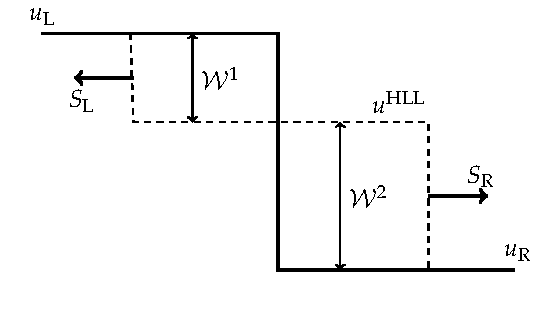
\includegraphics[width=0.47\textwidth,height=0.25\textwidth]
	{Figures/Theory/ScalarWaves-figure1.eps}}
	
	\captionsetup{justification=centering}
	
	\caption{Geometrical interpretation of how different numerical forms split the discontinuity.}
	\label{fig:FDS-waves}
\end{figure} 

Since the HLL-type scheme consists of two waves, we can write the updating formula for $ u_j^{n+1} $ in the wave propagation form (see~\cite[p.~80]{lev01}):
\begin{equation} \label{eq:scalar-W}
u_j^{n+1} = u_j - \frac{\Delta t}{\Delta x} \left( \sum_{p=1}^{2} S_{j-1/2}^{p,+} \mathcal{W}_{j-1/2}^p + \sum_{p=1}^{2} S_{j+1/2}^{p,-} \mathcal{W}_{j+1/2}^p \right), 
\end{equation}
where we introduce the notation $ S^{p,+} = \max \left( 0, S^p \right) $, $ S^{p,-} = \min \left( 0, S^p \right) $, and we define the wave velocities:
\begin{equation} \label{eq:scalar-W-S}
S_{j+1/2}^1 = \SLj, \quad S_{j+1/2}^2 = \SRj,
\end{equation}
and the waves:
\begin{equation} 
\mathcal{W}_{j+1/2}^1 = u_{j+1/2}^\text{HLL} - u_{j}, \quad \mathcal{W}_{j+1/2}^2 = u_{j+1} - u_{j+1/2}^\text{HLL}.
\end{equation}
For standard, one-parameter methods it is easy to show that:
\begin{align}
\ASj^- \Delta u_{j+1/2}
= & \frac{1}{2} \left( \lambda_{j+1/2} - \QSj \right) \Delta u_{j+1/2} \notag \\
= & \SLj \left( u_{j+1/2}^\text{HLL} - u_j \right) =
\sum_{p=1}^{2} S_{j+1/2}^{p,-} \mathcal{W}_{j+1/2}^p, \\
\ASj^+ \Delta u_{j+1/2}
= & \frac{1}{2} \left( \lambda_{j+1/2} + \QSj \right) \Delta u_{j+1/2} \notag \\
= & \SRj \left( u_{j+1} - u_{j+1/2}^\text{HLL} \right) =
\sum_{p=1}^{2} S_{j+1/2}^{p,+} \mathcal{W}_{j+1/2}^p.
\end{align}
This new framework provides a new insight into some properties of one-parameter methods. For standard-one parameter methods, \eqref{eq:scalar-W} becomes:
\begin{equation} \label{eq:scalar-W-oneQ}
u_j^{n+1} = u_j - \frac{\Delta t}{\Delta x} 
\left( 
Q_{\text{S},j-1/2} \left( u_{j} - u_{j-1/2}^\text{HLL} \right) - 
Q_{\text{S},j+1/2} \left( u_{j+1/2}^\text{HLL} - u_j \right) 
\right), 
\end{equation}
where by using \eqref{eq:HLL-NV-Qs} in \eqref{eq:scalar-uHLL} we have that an intermediate state of a one-parameter method is:
\begin{equation} \label{eq:scalar-uHLL1}
u_{j+1/2}^\text{HLL(1)} = \frac{1}{2} \left( u_{j} + u_{j+1} \right) - \frac{1}{2} \frac{\lambda_{j+1/2}}{\QSj}\left( u_{j+1} - u_j \right).
\end{equation}
By looking at \cref{fig:FDS-waves} we heuristically argue that the intermediate state of the one-parameter method should lie between the left and right state:
\begin{equation} \label{eq:scalar-waves-TVD}
u_{j+1/2}^\text{HLL(1)} \, \in \, \left[ \min \left( u_j, u_{j+1} \right), \max \left( u_j, u_{j+1} \right) \right].
\end{equation}
By enforcing this condition we find it is satisfied for:
\begin{equation} \label{eq:scalar-waves-lowerTVD}
\left| \lambda_{j+1/2} \right| \leq \QSj, \quad \forall \, j,
\end{equation}
which we recognize as the lower bound of the TVD condition \eqref{eq:3-NV-TVD}. We can see that in the wave propagation form, the upper bound of TVD condition limits how far can waves travel, while the lower bound limits the magnitude of the waves. We can show that \eqref{eq:scalar-waves-lowerTVD} implies \eqref{eq:scalar-waves-TVD} by rewriting \eqref{eq:scalar-waves-TVD} as:
\begin{align} 
u_j \geq u_{j+1/2}^\text{HLL(1)} \geq u_{j+1} \quad & \text{if} \quad u_{j} \geq u_{j+1}, \\
u_j \leq u_{j+1/2}^\text{HLL(1)} \leq u_{j+1} \quad & \text{if} \quad u_{j} \leq u_{j+1}.
\end{align}
We suppress the interface indices and observe that when $ u_{j} \geq u_{j+1} $, the left inequality can be rewritten as:
\begin{equation}
\frac{1}{2} \left( 1- \frac{\lambda}{Q_\text{S}} \right) \left( u_{j+1} - u_j \right) \leq 0.
\end{equation}
Since $ u_{j+1} - u_j \leq 0 $, we require that:
\begin{equation}
1 - \frac{\lambda}{Q_\text{S}} \geq 0.
\end{equation}
For $ \lambda > 0 $, we obtain that:
\begin{equation}
Q_\text{S} \geq |\lambda|,
\end{equation}
while for $ \lambda < 0 $ we obtain:
\begin{equation}
1 + \frac{|\lambda|}{Q_\text{S}} \geq 0,
\end{equation}
which is satisfied for any $ Q_\text{S} \geq 0 $. The remaining cases are done in the same way.

We can make several observation by considering $ u_{j+1/2}^\text{HLL(1)} $, eq. \eqref{eq:scalar-uHLL1}. The Roe scheme in flux-difference splitting form consists of a single discontinuity traveling either to the left or right, i.e. either $ A_\text{Roe}^{-} = 0 $ or $ A_\text{Roe}^{+} = 0 $. The wave propagation form consists of two waves traveling to the left and right, but it can be shown that by using $ Q_\text{Roe} $ in \eqref{eq:scalar-uHLL1} we obtain that either $ u_{j+1/2}^\text{HLL} = u_j $ or $ u_{j+1/2}^\text{HLL} = u_{j+1} $, hence one of the waves $ \mathcal{W} $ is equal to zero. This fits into the discussion above, since the Roe scheme is precisely the lower limit of the TVD condition.

Next, for the Lax-Wendroff scheme, $ Q_\text{L-W} = \lambda^2 \Delta t / \Delta x $, we obtain:
\begin{equation} 
u_{j+1/2}^\text{HLL-LW} = \frac{1}{2} \left( u_{j} + u_{j+1} \right) - \frac{1}{2} \frac{1}{\lambda} \frac{\Delta x}{\Delta t} \left( u_{j+1} - u_j \right),
\end{equation}
and the intermediate state is outside $ \mathcal{R} $, except when $ |\lambda|=\Delta x / \Delta t $.\footnote{Second-order accurate schemes are often achieved by using the \textit{wave limiters} which, as the name suggests, limit the magnitude of the waves $ \mathcal{W} $. Author conjectures that TVD wave limiters are precisely those that ensure that, at the discontinuities, the intermediate state lies within $ \mathcal{R} $.}

Further, in the case of transonic shock or transonic rarefaction when $ \lambda = 0 $, the Roe and Lax-Wendroff schemes do not have well defined intermediate state, since term $ \lambda/Q_\text{S} $ in \eqref{eq:scalar-uHLL1} becomes $ 0/0 $ and $ \Delta x /0 $, respectively.

Finally, we know that for the central scheme $ Q_\text{C} = 0 $. By using this in \eqref{eq:scalar-uHLL} the fraction on the right-hand side explodes, which explains why the scheme is unstable.

\subsection{Convergence and entropy stability}

We are now interested in convergence and entropy stability of the HLL-type scheme. As in previous chapter, we start by considering convergence to a weak solution along the lines of the Lax-Wendroff theorem. Then, we obtain stronger conditions to ensure convergence to the entropy solution.

\subsubsection*{Convergence}
The question of conservation was already discussed and we do not repeat it here. Consistency may be shown as earlier, by using the modified equation:
\begin{lemma}[Prebeg~\cite{cp2}] \label{lemma:HLL-consistent}
The HLL scheme with the numerical viscosity coefficient \eqref{eq:scalar-Q-HLL} is consistent with the scalar conservation law:
\begin{equation} \label{eq:SCL3}
u_t + f(u)_x = 0.
\end{equation}
\end{lemma}

\begin{proof}
Standard first-order methods give a second-order accurate approximation to the equation:
\begin{equation} \label{eq:3-ME3}
u_t + f(u)_x = \frac{1}{2} \frac{\Delta x^2}{\Delta t}\left[ \left( \frac{\Delta t}{\Delta x} \bar{Q} - c^2 \right) u_x \right]_x.
\end{equation}
By using \eqref{eq:scalar-Q-HLL} in \eqref{eq:3-ME3} we obtain that the HLL scheme gives a second-order accurate approximation to the equation:
\begin{equation} \label{eq:3-ME-HLL}
u_t + f(u)_x = \frac{1}{2} \frac{\Delta x^2}{\Delta t} \left[ D_{\text{HLL}} u_x \right]_x,
\end{equation}
where:
\begin{align}
D_{\text{HLL}} & = \frac{c - \CL}{\CR - \CL} \left( |\CR| - \CR^2 \right) \notag \\
& + \frac{\CR - c}{\CR - \CL} \left( |\CL|- \CL^2 \right) + \left( c - \CL \right) \left( \CR - c \right),
\end{align}
where $ \CL = \SL \Delta t / \Delta x $ and $ \CR = \SR \Delta t / \Delta x $. By keeping $ c = \text{const.} $ and passing $ \Delta x \rightarrow 0 $ we recover the scalar conservation law \eqref{eq:SCL3}.
\end{proof}

Next, we obtain conditions for the TVD stability:
\begin{lemma} \label{lemma:HLL-TVD}
The HLL scheme with the numerical viscosity coefficient \eqref{eq:scalar-Q-HLL} is TVD if:
\begin{equation} \label{eq:TVD-HLL-condition}
- \frac{\Delta x}{\Delta t} \leq
\SLj \leq 
\lambda_{j+1/2} \leq 
\SRj \leq
\frac{\Delta x}{\Delta t},
\quad \forall \, j.
\end{equation}
\end{lemma}

\begin{proof}
We suppress the interface indices and recall that a standard conservative scheme is unconditionally TVD if and only if:
\begin{equation}
\left| \lambda \right| \leq Q \leq \frac{\Delta x}{\Delta t},
\end{equation}
where for $ Q_{\text{HLL}} $ we require the following:
\begin{equation} \label{eq:TVD-HLL}
\left| \lambda \right| \leq \frac{\left| \SR \right| \left( \lambda - \SL \right) + \left| \SL \right| \left( \SR - \lambda \right)}{\SR - \SL} \leq \frac{\Delta x}{\Delta t}.
\end{equation}
The upper bound in \eqref{eq:TVD-HLL} can be rewritten as:
\begin{equation}
\left( \lambda - \SL \right) \left( |\SR|- \frac{\Delta x}{\Delta t} \right) + \left( \SR-\lambda \right) \left( |\SL|-\frac{\Delta x}{\Delta t} \right) \leq 0,
\end{equation}
which is always satisfied when the outer inequalities in \eqref{eq:TVD-HLL-condition} hold. The lower bound in \eqref{eq:TVD-HLL} can be rewritten as:
\begin{equation} 
\left( \lambda - \SL \right) \left( |\SR|- |\lambda| \right) + \left( \SR-\lambda \right) \left( |\SL|- |\lambda| \right) \geq 0, \label{eq:TVD-HLL-lower}
\end{equation}
which is always satisfied when the inner inequalities in \eqref{eq:TVD-HLL-condition} hold. \end{proof}

%We have the following result:
%\begin{proposition}
%The HLL scheme with the choice of wave velocities:
%\begin{equation} \label{eq:TVD-HLL-condition2}
%- \frac{\Delta x}{\Delta t} \leq
%\SLj \leq 
%\lambda_{j+1/2} \leq 
%\SRj \leq
%\frac{\Delta x}{\Delta t},
%\quad \forall \, j,
%\end{equation}
%converges to a weak solution of the scalar conservation law \eqref{eq:SCL2}.
%\end{proposition}
%
%\begin{proof}
%This follows from the Lax-Wendroff theorem, since the HLL scheme is conservative, consistent~(\Cref{lemma:HLL-consistent}) and TVD under the condition \eqref{eq:TVD-HLL-condition2}~(\Cref{lemma:HLL-TVD}).
%\end{proof}

\subsubsection*{Entropy stability}

%The convergence result above does not tell us if the scheme converges to the unique weak solution of the scalar conservation law. We can show that a scheme is entropy stable by using entropy functions, by showing that it is an E-scheme or by showing that it is monotone.

The TVD stability result above does not tell us if the scheme converges to the unique entropy-satisfying weak solution of the scalar conservation law. We can show that a scheme is entropy stable by using entropy functions, by showing that it is an E-scheme or by showing that it is monotone.

Herein, we will use entropy functions to show that the HLL scheme with the choice of the wave velocities according to Einfeldt~\cite{ein88}:
\begin{subequations} \label{eq:scalar-Einfeldt}
\begin{align}
\SL & = \min \left( \lambda_{j+1/2}, f'(u_j) \right), \\
\SR & = \max \left( \lambda_{j+1/2}, f'(u_{j+1}) \right),
\end{align}
\end{subequations}
is entropy stable.\footnote{In Einfeldt's paper~\cite{ein88}, the HLLE scheme is developed for the Euler equations. We will denote the choice \eqref{eq:scalar-Einfeldt} as the scalar HLLE because it is equivalent to applying the original Einfeldt's choice to the scalar conservation law.} Our proof closely follows the proof by Pelanti et al.~\cite[p.~12]{pel01} (see also~\cite{har83c,god96}).

We consider the discrete Riemann problem \eqref{eq:scalar-RP} for the scalar conservation law \eqref{eq:SCL2} with a convex flux function $ f(u) $. If the solution to the Riemann problem is supposed to be a shock \eqref{eq:scalar-shock}, the HLLE scheme yields $ \SL = \SR = \lambda $, and it can be shown that in the limit when $ \SL, \SR \rightarrow \lambda $, the HLLE scheme becomes the Roe scheme and the solution is:
\begin{equation} 
\widetilde{u}(x/t) = \left\{ \begin{array}{lll}
	u_\text{L} \quad & \text{if} \quad x < \lambda t, \\[0.25em]
	u_\text{R}		 & \text{if} \quad x > \lambda t. \end{array} \right.
\end{equation}
If the solution is supposed to be a rarefaction \eqref{eq:scalar-rarefaction}, the HLLE scheme yields $ \SL = f'(u_j) $ and $ \SR = f'(u_{j+1}) $, and the solution is:
\begin{equation} \label{eq:scalar-HLLE-r}
\widetilde{u}(x/t) = \left\{ \begin{array}{lll}
	u_\text{L}\quad & \text{if} \quad x < f'(u_\text{L}) t, \\[0.25em]
	u^\text{HLL}	& \text{if} \quad f'(u_\text{L}) t < x < f'(u_\text{R}) t, \\[0.25em]
	u_\text{R}      & \text{if} \quad x > f'(u_\text{R}) t. \end{array} \right.
\end{equation}
If the rarefaction is a \textit{transonic} rarefaction, i.e. \mbox{$ f'(u_\text{L}) < 0 <f'(u_\text{R}) $}, certain schemes (such as the Roe scheme) may lead to an entropy violation. If the HLLE scheme is entropy stable, the solution \eqref{eq:scalar-HLLE-r} must satisfy the integral form of the entropy condition \eqref{eq:SCL-entropy-inequality}:
\begin{equation} \label{eq:integral-EC}
\int_{0}^{\Delta t} \int_{-\frac{\Delta x}{2}}^{\frac{\Delta x}{2}} \left[ \eta (u)_t + \psi(u)_x \right] \diff x \diff t \leq 0.
\end{equation}
By using $ u = \widetilde{u}(x/t) $ and integrating \eqref{eq:integral-EC} we obtain:
\begin{equation}
\int_{-\frac{\Delta x}{2}}^{\frac{\Delta x}{2}} \eta (\widetilde{u}(x/\Delta t)) \diff x \leq 
\frac{\Delta x}{2} \left( \eta (u_\text{L}) + \eta (u_\text{R}) \right) - 
\Delta t \left( \psi(u_\text{R}) - \psi (u_\text{L}) \right).
\end{equation}
Since \eqref{eq:scalar-HLLE-r} consists of piecewise constant data, the left-hand side is:
\begin{align} \label{eq:HLLE-expanded}
\int_{-\frac{\Delta x}{2}}^{\frac{\Delta x}{2}} \eta (\widetilde{u}(x/ \Delta t)) \diff x
& = 
\eta(u^\text{HLL}) \left( \SR \Delta t - \SL \Delta t \right) \notag \\
& + \eta(u_\text{L}) \left( \SL \Delta t + \frac{\Delta x}{2} \right)
  + \eta(u_\text{R}) \left( \frac{\Delta x}{2} - \SR \Delta t \right). 
\end{align}
The outer bounds enclosing $ u^\text{HLL} $ in \eqref{eq:scalar-HLLE-r} are physical signal velocities that also appear in the exact solution \eqref{eq:scalar-rarefaction}, so we know from the conservation principle that $ u^\text{HLL} $ is equal to the integral of the exact solution $ u^\text{E}(x/t) $ from $ f'(u_\text{L}) \Delta t $ to $ f'(u_\text{R}) \Delta t $:
\begin{equation}
u^\text{HLL} = \frac{1}{\Delta t \left( \SR - \SL \right)} \int_{\SL \Delta t}^{\SR \Delta t} u^E(x/\Delta t) \diff x,
\end{equation}
where we used that $ \SL = f'(u_\text{L}) $ and $ \SR = f'(u_\text{R}) $ are the outer bounds of the exact solution \eqref{eq:scalar-rarefaction}. By using Jensen's inequality we have that:
\begin{equation} \label{eq:HLLE-Jensen}
\eta(u^\text{HLL}) \leq \frac{1}{\Delta t \left( \SR - \SL \right)} \int_{\SL t}^{\SR t} \eta(u^\text{E}(x/\Delta t)) \diff x .
\end{equation}
By using \eqref{eq:HLLE-Jensen} in \eqref{eq:HLLE-expanded} we obtain:
\begin{align}
\int_{-\frac{\Delta x}{2}}^{\frac{\Delta x}{2}} \eta (\widetilde{u}(x/\Delta t)) \diff x
& \leq 
\int_{\SL \Delta t}^{\SR \Delta t} \eta(u^\text{E}(x/ \Delta t)) \diff x \notag \\
& + \eta(u_\text{L}) \left( \SL t + \frac{\Delta x}{2} \right)
  + \eta(u_\text{R}) \left( \frac{\Delta x}{2} - \SR \Delta t \right),
\end{align}
where the right-hand side is the exact solution:
\begin{align}
\int_{-\frac{\Delta x}{2}}^{\frac{\Delta x}{2}} \eta (\widetilde{u}(x/\Delta t)) \diff x
& \leq
\int_{-\frac{\Delta x}{2}}^{\frac{\Delta x}{2}} \eta (u^\text{E}(x/\Delta t)) \diff x \notag \\
& \leq \frac{\Delta x}{2} \left( \eta (u_\text{L})
     + \eta (u_\text{R}) \right) - \Delta t \left( \psi(u_\text{R}) - \psi (u_\text{L}) \right),
\end{align}
where the last inequality follows from the fact that the exact solution satisfies the entropy inequality. Hence, we showed that the HLLE scheme is entropy stable, provided that the TVD condition \eqref{eq:TVD-HLL-condition} is satisfied.

\subsection{LTS-HLL scheme for scalar conservation laws}

In addition to the numerical viscosity and the flux-difference splitting form, we recall that it was also possible to write the updating formula of a standard method in terms of the solutions to the neighboring Riemann problems (see \eqref{eq:convex-update}):
\begin{equation} \label{eq:convex-update2}
u_j^{n+1} =
\frac{1}{\Delta x}
\int_{0}^{\frac{\Delta x}{2}} \widetilde{u}_{j-1/2} \left( x/ \Delta t \right) \diff x +
\frac{1}{\Delta x}
\int_{-\frac{\Delta x}{2}}^{0} \widetilde{u}_{j+1/2} \left( x/ \Delta t \right) \diff x,
\end{equation}
where $ \widetilde{u}_{j-1/2}(x/t) $ is the approximate solution to the local Riemann problem at the cell interface $ x_{j-1/2} $. Since in LTS method the value of $ u_j^{n+1} $ may depend on more than three cells, it might also depend on more than two Riemann problems. Following LeVeque~\cite{lev85} (see also Lindqvist et al.~\cite{lin16}) we may write the general updating formula of LTS method in terms of solutions to all Riemann problems in the domain of dependence:
\begin{equation} \label{eq:scalar-LTS-update}
u_j^{n+1} = \frac{\Delta t}{\Delta x} \sum\limits_{i=-\infty}^{\infty} \int_{(i-1)\frac{\Delta x}{\Delta t}}^{i \frac{\Delta x}{\Delta t}} \widetilde{u}_{j+1/2-i} \diff \xi_i - \sum\limits_{l=-\infty}^{\infty} u_l,
\end{equation}
where $ \widetilde{u}_{j+1/2-i} $ is the solution to the Riemann problem at $ x_{j+1/2-i} $ and:
\begin{equation}
\xi_i = \frac{x - x_{j+1/2-i}}{t - t^n}.
\end{equation}
We note that \eqref{eq:scalar-LTS-update} reduces to \eqref{eq:convex-update2} when $ \bar{C} \leq 1 $.

To obtain the numerical viscosity and flux-difference splitting coefficients of the LTS-HLL scheme, we follow our paper~\cite{jp2} and use \eqref{eq:scalar-RP-HLL} in \eqref{eq:scalar-LTS-update} to determine the flux-difference splitting coefficients, and then use the formula \eqref{eq:FDS-NV} to directly obtain the numerical viscosity coefficients. For a slightly different approach, which includes geometrical consideration and more heuristic arguments we also refer to our paper~\cite{jp2}, where as the starting point we used HLL(C) schemes for systems of equations.

\begin{proposition}[Prebeg et al.~\cite{jp2}] \label{prop:LTS-HLL-A}
The LTS-HLL scheme can be written in the flux-difference splitting form \eqref{eq:scalar-LTS-FDS} with coefficients:
\begin{align} \label{eq:scalar-LTS-HLL-A}
A_\text{HLL}^{i\pm} = & \pm \frac{\lambda - \SL}{\SR - \SL} \max \left( 0, \min \left( \pm \SR - i \frac{\Delta x}{\Delta t}, \frac{\Delta x}{\Delta t} \right) \right) \notag \\
& \pm \frac{\SR - \lambda}{\SR - \SL} \max \left( 0, \min \left( \pm \SL - i \frac{\Delta x}{\Delta t}, \frac{\Delta x}{\Delta t} \right) \right). 
\end{align}
\end{proposition}

\begin{proof}
The HLL Riemann solver \eqref{eq:scalar-RP-HLL} can be written as:
\begin{subequations}
\begin{align}
\widetilde{u}_{j+1/2}(\zeta) & = u_j + H(\zeta - \SL) \left( u_{j+1/2}^\text{HLL} - u_j \right) + H( \zeta - \SR) \left( u_{j+1} - u_{j+1/2}^\text{HLL} \right) \\
&=u_{j+1}-H(\SL-\zeta)\left(u_{j+1/2}^\text{HLL}-u_j\right)-H(\SR-\zeta)\left(u_{j+1}-u_{j+1/2}^\text{HLL}\right),
\end{align}
\end{subequations}
where $H$ is the Heaviside function. By using \eqref{eq:scalar-uHLL} we can rewrite this as:
\begin{subequations}
\begin{align}
\widetilde{u}_{j+1/2}(\zeta) 
& = 
u_j +
\left( \frac{H(\zeta-\SL)}{\SR-\SL}(\SR-\lambda) +
\frac{H(\zeta-\SR)}{\SR-\SL}(\lambda-\SL)
\right) (u_{j+1}-u_j) \label{eq:uzeta-a} \\
& = u_{j+1} -
\left( \frac{H(\SL-\zeta)}{\SR-\SL}(\SR-\lambda) +
\frac{H(\SR-\zeta)}{\SR-\SL}(\lambda-\SL)
\right)(u_{j+1}-u_j). \label{eq:uzeta-b}
\end{align}
\end{subequations}
We then use \eqref{eq:uzeta-a} in \eqref{eq:scalar-LTS-update} and note that for $i\leq 0$ we can write:
\begin{equation}\label{eq:negi}
\int_{(i-1)\frac{\Delta x}{\Delta t}}^{i\frac{\Delta x}{\Delta t}} \widetilde{u}_{j+1/2-i} (\zeta_i) \diff \zeta_i = 
\frac{\Delta x}{\Delta t} u_{j-i}-A_{j+1/2-i}^{(-i)-}\left(u_{j+1-i}-u_{j-i}\right),
\end{equation}
where $ A^{i-} $ is the flux-difference splitting coefficient:
\begin{align}\label{eq:scalar-HLL-Aminus}
A_\text{HLL}^{i-} & = \frac{\lambda - \SL}{\SR - \SL} \min \left( 0, \max \left( \SR + i \frac{\Delta x}{\Delta t}, -\frac{\Delta x}{\Delta t} \right) \right) \notag \\
& + \frac{\SR - \lambda}{\SR - \SL} \min \left( 0, \max \left( \SL + i \frac{\Delta x}{\Delta t}, -\frac{\Delta x}{\Delta t} \right) \right). 
\end{align}
Similarly, we use \eqref{eq:uzeta-b} in \eqref{eq:scalar-LTS-update} and note that for $i\geq 1$ we can write:
\begin{equation}\label{eq:posi}
\int_{(i-1)\frac{\Delta x}{\Delta t}}^{i\frac{\Delta x}{\Delta t}} \widetilde{u}_{j+1/2-i} (\zeta_i)\diff \zeta_i=\frac{\Delta x}{\Delta t}u_{j+1-i}- A_{j+1/2-i}^{(i-1)+}\left(u_{j+1-i}-u_{j-i}\right),
\end{equation}
where $ A^{i+} $ is the flux-difference splitting coefficient:
\begin{align}\label{eq:scalar-HLL-Aplus}
A_\text{HLL}^{i+} & = \frac{\lambda - \SL}{\SR - \SL} 
\max \left( 0, \min \left( \SR - i \frac{\Delta x}{\Delta t}, \frac{\Delta x}{\Delta t} \right) \right) \notag \\
& + \frac{\SR - \lambda}{\SR - \SL} 
\max \left( 0, \min \left( \SL - i \frac{\Delta x}{\Delta t}, \frac{\Delta x}{\Delta t} \right) \right). 
\end{align}
Substituting \eqref{eq:negi} and \eqref{eq:posi} into \eqref{eq:scalar-LTS-update} we recover the LTS method in the flux-difference splitting form \eqref{eq:scalar-LTS-FDS}.
\end{proof}

\begin{proposition}[Prebeg et al.~\cite{jp2}]
The LTS-HLL scheme can be written in the numerical viscosity form \eqref{eq:scalar-LTS-NV} with coefficients:
\begin{subequations} \label{eq:scalar-LTS-HLL-Q}
\begin{align}
Q_\text{HLL}^0 & = \frac{\left| \SR \right| \left( \lambda - \SL \right) + \left| \SL \right| \left( \SR - \lambda \right) }{\SR - \SL}, \\
Q_\text{HLL}^{\mp i} & = 2 \frac{\lambda - \SL}{\SR - \SL} \max \left( 0, \pm \SR - i \frac{\Delta x}{\Delta t} \right) \notag \\
& + 2 \frac{\SR - \lambda}{\SR - \SL} \max \left( 0, \pm \SL - i \frac{\Delta x}{\Delta t} \right) \quad \text{for} \quad i>0. 
\end{align} 
\end{subequations}
\end{proposition}

\begin{proof}
Use \eqref{eq:scalar-LTS-HLL-A} in \eqref{eq:FDS-NV} to recover \eqref{eq:scalar-LTS-HLL-Q}.
\end{proof}

In addition to NV and FDS form, we may also write the LTS-HLL scheme in the wave propagation form \eqref{eq:scalar-W}:
\begin{equation} \label{eq:scalar-LTS-W}
u_j^{n+1} = u_j - \frac{\Delta t}{\Delta x} \sum\limits_{i=0}^{\infty} \left( \sum\limits_{p=1}^{2} S_{j-1/2-i}^{p,i+} \mathcal{W}_{j-1/2-i}^p + \sum\limits_{p=1}^{2} S_{j+1/2+i}^{p,i-} \mathcal{W}_{j+1/2+i}^p \right),
\end{equation}
where we recall that $ S^1 = \SL $ and $ S^2 = \SR $ (eq. \eqref{eq:scalar-W-S}). The wave velocities \eqref{eq:scalar-W-S} are modified as:
\begin{equation} \label{eq:scalar-LTS-W-S}
S^{p,i\pm} = \pm \max \left( 0, \min \left( \pm S^p - i \frac{\Delta x}{\Delta t}, \frac{\Delta x}{\Delta t} \right) \right).
\end{equation}
We recall that the interface indices on $ A $, $ Q $ and $ S^p $ have been suppressed, and we refer to \cref{rem:indexing} (p.~\pageref{eq:scalar-LTS-Roe-NV}) for explanation of the notation.

\subsection{A class of LTS one-parameter methods}
\label{cha3:sec:LTS-one-parameter}

In \Cref{prop:HLL-NV-Qs,prop:HLL-FDS-As} we showed that the standard one-parameter methods \eqref{eq:scalar-Q} and \eqref{eq:scalar-A} can be deduced from the HLL-type scheme by appropriate choice of $ \SL $ and $ \SR $. This motivated the question if we can obtain LTS one-parameter methods from the the LTS-HLL-type scheme by appropriate choice of $ \SL $ and $ \SR $. 

We begin with the LTS-Roe and LTS-Lax-Friedrichs schemes because we already have their NV and FDS coefficients. We may recover the LTS-Roe scheme in the NV \eqref{eq:scalar-LTS-Roe-NV} and FDS \eqref{eq:scalar-LTS-Roe-FDS} form by using:
\begin{equation}
\SL = - Q_\text{Roe}, \quad \SR = Q_\text{Roe},
\end{equation}
in the LTS-HLL-type scheme in the NV \eqref{eq:scalar-LTS-HLL-Q} and FDS \eqref{eq:scalar-LTS-HLL-A} form, respectively. In order to obtain the LTS-Lax-Friedrichs scheme in the NV \eqref{eq:scalar-LTS-LxF-NV} and FDS \eqref{eq:scalar-LTS-LxF-FDS} form, we must use:
\begin{equation}
\SL = - k Q_\text{LxF}, \quad \SR = k Q_\text{LxF},
\end{equation}
in the LTS-HLL-type scheme in the NV \eqref{eq:scalar-LTS-HLL-Q} and FDS \eqref{eq:scalar-LTS-HLL-A} form, respectively. This illuminates an important point related to the Lax-Friedrichs scheme. The numerical viscosity coefficient of the standard Lax-Friedrichs scheme \eqref{eq:scalar-Q-LxF} was defined as:
\begin{equation} \label{eq:scalar-Q-LxF1}
Q_\text{LxF} = \Delta x / \Delta t,
\end{equation}
while the partial numerical viscosity coefficient of the LTS-Lax-Friedrichs scheme \eqref{eq:scalar-LTS-LxF-NV} associated with $ i=0 $ was defined as:
\begin{equation} \label{eq:scalar-LTS-LxF-Q0}
Q_\text{LTS-LxF}^0 = k \Delta x / \Delta t.
\end{equation}
In order to obtain the LTS-Lax-Friedrichs scheme \eqref{eq:scalar-LTS-LxF-NV} from the LTS-HLL-type scheme \eqref{eq:scalar-LTS-HLL-Q}, we must use \eqref{eq:scalar-LTS-LxF-Q0}. We can now see that in the standard Lax-Friedrichs scheme \eqref{eq:scalar-Q-LxF1} the coefficient $ k=1 $ is implicitly assumed, and that the numerical viscosity coefficient of the standard method in fact reads $ Q_\text{LxF} = k \Delta x / \Delta t $.

Having obtained the LTS-Roe and LTS-Lax-Friedrichs schemes by following the approach used for standard methods (see \Cref{prop:HLL-NV-Qs,prop:HLL-FDS-As}), we establish equivalent results for other LTS methods.

\begin{proposition}\label{prop:LTS-HLL-NV-Qs}
Consider a first-order accurate, LTS one-parameter conservative scheme written in the numerical viscosity form \eqref{eq:scalar-LTS-NV}, which is uniquely determined by the partial numerical viscosity coefficients $ Q_\text{S}^i $. By defining $ \SL $ and $ \SR $ in the LTS-HLL-type scheme \eqref{eq:scalar-LTS-HLL-Q} as:
\begin{equation} \label{eq:LTS-HLL-NV-Qs}
\SL = -Q_\text{S}, \quad \SR = Q_\text{S},
\end{equation}
the numerical viscosity coefficients of the HLL-type scheme become:
\begin{subequations} \label{eq:scalar-LTS-NV-oneQ}
\begin{align}
Q_\text{HLL}^0 & = Q_\text{S}, \\
Q_\text{HLL}^{\mp i} & = \frac{\lambda - Q_\text{S}}{Q_\text{S}} \max \left( 0, \pm Q_\text{S} - i \frac{\Delta x}{\Delta t} \right) \notag \\
& +\frac{Q_\text{S} - \lambda}{Q_\text{S}} \max \left( 0, \mp Q_\text{S} - i \frac{\Delta x}{\Delta t} \right) \quad \text{for}\quad i>0. 
\end{align} 
\end{subequations}
\end{proposition}

\begin{proof}
Use \eqref{eq:LTS-HLL-NV-Qs} in \eqref{eq:scalar-LTS-HLL-Q} to obtain \eqref{eq:scalar-LTS-NV-oneQ}.
\end{proof}

\begin{proposition}\label{prop:LTS-HLL-FDS-As}
Consider a first-order accurate, LTS one-parameter conservative scheme written in the flux-difference splitting form \eqref{eq:scalar-LTS-FDS}, which is uniquely determined by the flux-difference splitting coefficients $ A_\text{S}^{i\pm} $. By defining $ \SL $ and $ \SR $ in the LTS-HLL-type scheme \eqref{eq:scalar-LTS-HLL-Q} as:
\begin{equation} \label{eq:LTS-HLL-FDS-As}
\SL = A_\text{S}^- - A_\text{S}^+ = - Q_\text{S}, \quad \SR = A_\text{S}^+ - A_\text{S}^- = Q_\text{S},
\end{equation}
the flux-difference splitting coefficients of the HLL-type scheme become:
\begin{align} \label{eq:scalar-LTS-FDS-oneA}
A_\text{S}^{i\pm} = & \pm \frac{\lambda + Q_\text{S}}{2 Q_\text{S}} \max \left( 0, \min \left( \pm Q_\text{S} - i \frac{\Delta x}{\Delta t}, \frac{\Delta x}{\Delta t} \right) \right) \notag \\
& \pm \frac{Q_\text{S} - \lambda}{2 Q_\text{S}} \max \left( 0, \min \left( \mp Q_\text{S} - i \frac{\Delta x}{\Delta t}, \frac{\Delta x}{\Delta t} \right) \right). 
\end{align}
\end{proposition}

\begin{proof}
Use \eqref{eq:LTS-HLL-FDS-As} is \eqref{eq:scalar-LTS-HLL-A} to obtain \eqref{eq:scalar-LTS-FDS-oneA}.
\end{proof}

We obtained a framework of LTS two-parameter methods that contains already existing LTS-Roe and LTS-Lax-Friedrichs schemes, and allows us to directly obtain an LTS extension of any first-order accurate standard one-parameter method. We note that an LTS extension of standard method is not unique. In our framework, what makes an LTS method an extension of a standard method is the fact that they are based on the same NV (or FDS) coefficients, and that the LTS method reduces to the standard method for $ \bar{C} \leq 1 $. Newly developed LTS extensions include:
\begin{itemize} \label{eq:LTS-1p-itemize}
\item \textit{LTS-Engquist-Osher:} Framework established above provides an LTS extension of the Engquist-Osher scheme. In the next section, we will show that our LTS-Engquist-Osher scheme is not entropy stable. On the other hand, Brenier~\cite{bre84} developed a monotone (hence entropy stable) LTS-Engquist-Osher scheme. Unfortunately, we do not know NV or FDS coefficients of the LTS-Engquist-Osher scheme by Brenier so at the moment we cannot compare these two.

\item \textit{LTS-Godunov:} Using $ \SL=-Q_\text{God} $ and $ \SR=Q_\text{God} $ does not recover the LTS-Godunov scheme of Lindqvist et al.~\cite{lin16}. In our framework, every scheme can be interpreted as the two-wave Riemann solver~\eqref{eq:scalar-RP-HLL}, and that also applies to our LTS-Godunov scheme when the solution is supposed to be a rarefaction. On the other hand, the LTS-Godunov scheme of Lindqvist et al.~\cite{lin16} splits a rarefaction into as many waves necessary to resolve it exactly (to projection error) on the given grid.

\item \textit{LTS-Lax-Wendroff:} \Cref{prop:LTS-HLL-NV-Qs,prop:LTS-HLL-FDS-As} are stated for first-order accurate schemes. A straightforward LTS extension of the Lax-Wendroff scheme seems to be unstable. This issue is currently being investigated, and as a possible cause of failure we note that for standard methods we have:
\begin{equation}
c^2 \leq |c| \leq 1 \quad \rightarrow \quad Q_\text{L-W} \leq Q_\text{Roe} \leq Q_\text{LxF}.
\end{equation}
However, for LTS methods with an arbitrary Courant number, the numerical viscosity coefficient of the Lax-Wendroff scheme may exceed both $ Q_\text{Roe} $ and $ Q_\text{LxF} $.
\end{itemize}

\subsection{Convergence and entropy stability}
\label{sec:LTS-HLL:C-ES-scalar-LTS}

\subsubsection*{Convergence} 

All considerations regarding the convergence of existing LTS methods (see section~\ref{sec:Background:C-ES-scalar-LTS}) also apply to LTS-HLL-type schemes. Namely, following the Lax-Wendroff theorem we are able to show that LTS-HLL-type methods with certain restrictions on the wave velocity estimates $ \SL $ and $ \SR $ converge to a weak solution.

The question of conservation was already discussed and we do not repeat it here. Consistency may be shown as earlier, by using the modified equation:
\begin{lemma}[Prebeg~\cite{cp2}] \label{lemma:LTS-HLL-consistent}
The LTS-HLL scheme with the numerical viscosity coefficient \eqref{eq:scalar-LTS-HLL-Q} is consistent with the scalar conservation law:
\begin{equation} \label{eq:SCL4}
u_t + f(u)_x = 0.
\end{equation}
\end{lemma}

\begin{proof}
First-order methods give a second-order accurate approximation to the equation:
\begin{equation} \label{eq:LTS-ME3}
u_t + f(u)_x = \frac{1}{2} \frac{\Delta x^2}{\Delta t} \left[ \left( \sum\limits_{i=1-k}^{k-1} \frac{\Delta t}{\Delta x} \bar{Q}^i - c^2 \right) u_x \right]_x.
\end{equation}
By using \eqref{eq:scalar-LTS-HLL-Q} in \eqref{eq:LTS-ME3} we obtain that the LTS-HLL scheme gives a second-order accurate approximation to the equation:
\begin{equation} \label{eq:LTS-ME-HLL}
u_t + f(u)_x = \frac{1}{2} \frac{\Delta x^2}{\Delta t} \left[ D_{\text{LTS-HLL}} u_x \right]_x,
\end{equation}
where:
\begin{align}
D_\text{LTS-HLL} & = \frac{c - \CL}{\CR - \CL} \left( \lceil |\CR| \rceil - |\CR| \right) \left( 1 + |\CR| - \lceil |\CR| \rceil \right) \notag \\ 
& + \frac{\CR - c}{\CR - \CL} \left( \lceil |\CL| \rceil - |\CL| \right) \left( 1 + |\CL| - \lceil |\CL| \rceil \right) \notag \\ 
& + \left( c - \CL \right) \left( \CR - c \right),
\end{align}
where $ \CL = \SL \Delta t / \Delta x $, $ \CR = \SR \Delta t / \Delta x $, and $ \lceil c \rceil = \min \{ n \in \mathbb{Z} \,| \, n \geq c \} $ is a ceiling function. By keeping $ c = \text{const.} $ and passing $ \Delta x \rightarrow 0 $ we recover the scalar conservation law \eqref{eq:SCL4}.
\end{proof}

To show TVD stability we use the TVD conditions for the LTS method in terms of the numerical viscosity coefficients, see \eqref{eq:LTS-TVD}.

\begin{lemma} \label{lemma:LTS-HLL-TVD}
The LTS-HLL scheme with the numerical viscosity coefficients \eqref{eq:scalar-LTS-HLL-Q} is TVD if:
\begin{equation} \label{eq:LTS-HLL-TVD}
\SLj \leq \lambda_{j+1/2} \leq \SRj, \quad \forall \, j.
\end{equation}
\end{lemma}

\begin{proof}
We suppress the interface indices and note that by substituting \eqref{eq:scalar-LTS-HLL-Q} in \eqref{eq:LTS-TVD-a}--\eqref{eq:LTS-TVD-c} the TVD conditions become:
\begin{subequations}
\begin{align}
  \left( \lambda - \SL \right) \left( \frac{\Delta x}{\Delta t} - \min \left( \left| \SR \right|, \frac{\Delta x}{\Delta t} \right) \right) & \notag \\ 
+ \left( \SR - \lambda \right) \left( \frac{\Delta x}{\Delta t} - \min \left( \left| \SL \right|, \frac{\Delta x}{\Delta t} \right) \right) 
& \geq 0, \\
  \left( \lambda - \SL \right) \max \left( 0, \min \left( \pm 2 \SR, 4 \frac{\Delta x}{\Delta t} \mp 2\SR \right) \right) \notag \\
+ \left( \SR - \lambda \right) \max \left( 0, \min \left( \pm 2 \SL, 4 \frac{\Delta x}{\Delta t} \mp 2\SL \right) \right)
& \geq 0, \\
  \left( \lambda - \SL \right) \max \left( 0, \min \left( \pm \SR - i \frac{\Delta x}{\Delta t}, \mp \SR + i \frac{\Delta x}{\Delta t} + 2 \right) \right) & \notag \\
+ \left( \SR - \lambda \right) \max \left( 0, \min \left( \pm \SL - i \frac{\Delta x}{\Delta t}, \mp \SL + i \frac{\Delta x}{\Delta t} + 2 \right) \right) & \geq 0 \quad \forall \quad i \geq 1,
\end{align}
\end{subequations}
which are always satisfied under the condition \eqref{eq:LTS-HLL-TVD}.
\end{proof}

%We have the following result:
%\begin{proposition}
%The LTS-HLL scheme with the choice of wave velocities:
%\begin{equation} \label{eq:TVD-LTS-HLL-condition}
%\SLj \leq \lambda_{j+1/2} \leq \SRj, \quad \forall \, j,
%\end{equation}
%converges to a weak solution of the scalar conservation law \eqref{eq:SCL4}.
%\end{proposition}
%
%\begin{proof}
%This follows from the Lax-Wendroff theorem, since the LTS-HLL scheme is conservative, consistent~(\Cref{lemma:LTS-HLL-consistent}) and TVD under the condition \eqref{eq:TVD-LTS-HLL-condition}~(\Cref{lemma:LTS-HLL-TVD}).
%\end{proof}

\subsubsection*{Entropy stability}

The discussion on entropy stability of existing LTS methods from \cref{sec:Background:C-ES-scalar-LTS} also applies here. We note that in general, the class of TVD LTS-HLL-type schemes is not entropy stable, because this class includes the entropy violating LTS-Roe scheme. We will address the question of entropy stability in LTS methods in \cref{sec:EV-ME} by using the modified equation analysis.

\subsection{LTS-HLL(C) schemes for systems of conservation laws}

The LTS-HLL-type schemes can be extended to systems of equations following the same way the already existing LTS methods have been extended to systems of equations, see~\cref{sec:Background:FVM-systems}. A slightly different approach to obtain the LTS-HLL scheme for systems of equations is given in our paper~\cite{jp2}, where we start with the standard HLL(C) schemes for systems of equations and extend them to the LTS framework. Our paper~\cite{jp2} also includes analysis of numerical diffusion in the LTS-HLL scheme for the Euler equations, and numerical results for both LTS-HLL(C) schemes applied to the Euler equations.

Up to now, we did not explicitly present the HLLC and the LTS-HLLC schemes. This is due to the fact that we did not develop a scalar counterpart of the HLLC scheme, and because the HLLC scheme does not naturally fit into the NV and FDS form. Nevertheless, an LTS-HLLC scheme in a conservation form can be obtained in a relatively straightforward manner and we refer to our papers~\cite{cp2,jp2} for more details.

Herein, we show that both LTS-HLL(C) schemes for systems of equations can be also written in the wave propagation form. This can be done by combining elements of wave propagation form and the HLLC scheme, as is done for instance by Pelanti and Shyue~\cite{pel14}. We skip technical details and give a final result.

An LTS scheme for scalar conservation law in the wave propagation form \eqref{eq:scalar-LTS-W} can be extended to systems of equations as:
\begin{equation} \label{eq:system-LTS-W}
\mathbf{U}_j^{n+1} = \mathbf{U}_j - 
\frac{\Delta t}{\Delta x} \sum\limits_{i=0}^{\infty} \left(
\sum\limits_{p=1}^{m} S_{j-1/2-i}^{p,i+} \mathcal{W}_{j-1/2-i}^p +
\sum\limits_{p=1}^{m} S_{j+1/2+i}^{p,i-} \mathcal{W}_{j+1/2+i}^p 
\right),
\end{equation}
where for the HLL scheme $ m=2 $, and the wave velocities are:
\begin{equation}
S^1 = S, \quad S^2 = \SR,
\end{equation}
while the waves are:
\begin{subequations}
\begin{align}
\mathcal{W}_{j-1/2}^1 & = \mathbf{U}_{j-1/2}^\text{HLL} - \mathbf{U}_{j-1}, \quad \\
\mathcal{W}_{j-1/2}^2 & = \mathbf{U}_{j} - \mathbf{U}_{j-1/2}^\text{HLL},
\end{align}
\end{subequations}
where $ \mathbf{U}_{j-1/2}^\text{HLL} $ is determined following the same principles as for the intermediate state in case of scalar conservation law \eqref{eq:scalar-uHLL}. For the HLLC scheme applied to one-dimensional Euler equations $ m=3 $, and the wave velocities are:
\begin{equation}
S^1 = \SL, \quad S^2 = S_\text{C}, \quad S^3 = \SR,
\end{equation}
while the waves are:
\begin{subequations}
\begin{align}
\mathcal{W}_{j-1/2}^1 & = \mathbf{U}_{\text{L},j-1/2}^\text{HLLC} - \mathbf{U}_{j-1}, \quad \\
\mathcal{W}_{j-1/2}^2 & = \mathbf{U}_{\text{R},j-1/2}^\text{HLLC} - \mathbf{U}_{\text{L},j-1/2}^\text{HLLC}, \quad \\
\mathcal{W}_{j-1/2}^3 & = \mathbf{U}_{j}^\text{HLLC} - \mathbf{U}_{\text{R},j-1/2}^\text{HLLC},
\end{align}
\end{subequations}
where the definition of the contact wave velocity $ S_\text{C} $ and the intermediate states $ \mathbf{U}_{\text{L,R},j-1/2}^\text{HLLC} $ can be found in our papers~\cite{cp2,jp2} and in paper by Toro et al.~\cite{tor94} and the book by Toro~\cite{tor09}, from where we adopted them. All velocities are modified in the same manner as:
\begin{equation} \label{eq:system-LTS-W-S}
S_\text{L,C,R}^{i\pm} = \pm \max \left( 0, \min \left( \pm S_\text{L,C,R} - i \frac{\Delta x}{\Delta t}, \frac{\Delta x}{\Delta t} \right) \right).
\end{equation}

\subsection{Choice of the wave velocity estimates $ \SL $ and $ \SR $}
\label{s:SLSR}

We now address the question on how to choose the wave velocity estimates $ \SL $ and $ \SR $. This question was left open in the original paper where the HLL scheme was introduced~\cite{har83a}, and was addressed by a number of authors in the coming years, see beginning of~\cref{sec:LTS-HLL(C)}. Herein, we outline some of velocity choices as applied to systems of equations, and we note that all of these also apply to the HLLC scheme and to the LTS extensions of the HLL(C) schemes.

We have already seen that for the scalar conservation laws, we can recover standard one-parameter methods from the standard HLL-type framework by an appropriate choice of $ \SL $ and $ \SR $. In addition, we constructed genuinely two-parameter HLLE scheme. For systems of conservation laws, we can exactly deduce one-parameter methods from the HLL-type framework only for systems with two equations. If system of equations has more than two equations, we can exactly deduce only those one-parameter methods which consist of two waves (such as the Lax-Friedrichs scheme), but not those schemes that consist of more than two waves (such as the Roe scheme). 

For example, by defining:
\begin{equation} \label{eq:system-SLSR-LxF}
\SLj = - k \Delta x / \Delta t, \qquad \SRj = k \Delta x / \Delta t,
\end{equation}
we obtain the eigenvalues $ (\omega^1,\dots,\omega^N) $ and $ (\lambda^1,\dots,\lambda^N) $ corresponding to the Lax-Friedrichs scheme, and by defining:
\begin{equation}
\SLj = -\SRj, \qquad
\SRj = \max ( |\lambda_j^1|,|\lambda_{j+1}^1|,|\lambda_j^N|,|\lambda_{j+1}^N| ),
\end{equation}
we obtain the eigenvalues $ (\omega^1,\dots,\omega^N) $ and $ (\lambda^1,\dots,\lambda^N) $ corresponding to the Rusanov scheme. We note that we will obtain genuine Lax-Friedrichs and Rusanov schemes independent of how many waves the system of equations has. By choosing:
\begin{equation} \label{eq:system-SLSR-Roe}
\SLj = \lambda_{\text{Roe},j+1/2}^1, \qquad
\SRj = \lambda_{\text{Roe},j+1/2}^N,
\end{equation}
we obtain the eigenvalues $ (\omega^1,\omega^N) $ and $ (\lambda^1,\lambda^N) $ corresponding to the Roe scheme. The choice \eqref{eq:system-SLSR-Roe} identically reduces to the Roe scheme only for systems with two waves. For standard methods, the above was observed already by Davis~\cite{dav88} and Einfeldt~\cite{ein88}.

Some other choices are given as:
\begin{equation} \label{eq:system-Davis1}
\left. \begin{array}{ll}
S_{\text{L},j+1/2} = \lambda_j^1 \\[0.5em]
S_{\text{R},j+1/2} = \lambda_{j+1}^N \end{array} \right. \qquad \text{Davis \#1~\cite{dav88}}.
\end{equation}
\begin{equation} \label{eq:system-Davis2}
\left. \begin{array}{ll}
S_{\text{L},j+1/2} = \min \left( \lambda_j^1,   \lambda_{j+1}^1 \right) \\[0.5em]
S_{\text{R},j+1/2} = \max \left( \lambda_{j}^N, \lambda_{j+1}^N \right) \end{array} \right. \qquad \text{Davis \#2~\cite{dav88}}.
\end{equation}
\begin{equation} \label{eq:system-Einfeldt}
\left. \begin{array}{ll}
S_{\text{L},j+1/2} = \min \left( \lambda_j^1, \lambda_{j+1/2}^1 \right) \\[0.5em]
S_{\text{R},j+1/2} = \max \left( \lambda_{j+1/2}^N, \lambda_{j+1}^N \right) \end{array} \right. \qquad \text{Einfeldt~\cite{ein88}}.
\end{equation} More complicated choices constructed for the Euler equations can be found in Toro et al.~\cite{tor94} and Bouchut~\cite{bou04}, where Bouchut developed a special choice of $ \SL $ and $ \SR $ in order to handle vacuum in the Euler equations. 

The choice of the wave velocities according to Einfeldt~\cite{ein88} is very popular among the standard methods, because it yields an entropy stable and a positivity preserving scheme~\cite{ein91}. Among the choices \eqref{eq:system-Davis1}--\eqref{eq:system-Einfeldt} and those found in Toro et al.~\cite{tor94}, Einfeldt's choice \eqref{eq:system-Einfeldt} was also found to yield the very best results when used in LTS-HLL(C) schemes. These observations are based on our experience, and more rigorous comparison may be fruitful.

The LTS-HLLE scheme for systems of equations seems to inherit the HLLE scheme property of being entropy stable, but does not inherit the HLLE scheme property of being positivity preserving. The former will be addressed in the next~\cref{sec:EV-ME}~\textit{Entropy stability} and it is a topic of our conference paper~\cite{cp2}, while the latter will be addressed in~\cref{sec:PP}~\textit{Positivity preservation} and it is a topic of our journal paper~\cite{jp3}. 

%
\section{Entropy stability}
\label{sec:EV-ME}

Earlier in the thesis (\cref{sec:Background:C-ES-scalar-LTS,sec:LTS-HLL:C-ES-scalar-LTS}), we have seen that the tools commonly used to prove entropy stability of standard methods are not readily available for LTS methods. Therein, we postponed the discussion on entropy stability in LTS methods, and now we finally address it by using modified equation. We begin this section with a word of caution:
\begin{quote}
\small
\textit{"Modified equations have been a commonly used tool in the study of difference schemes. Because of the lack of any theoretical foundation, this use has been accompanied by constant difficulties and results derived from modified equations have sometimes been
regarded with apprehension. As a result, a situation arises where authors either
disregard entirely the technique or have an unjustified faith in its scope."}
\qauthor{Griffiths and Sanz-Serna~\cite{gri86}}
\end{quote}
\vspace{-2.5mm}
We are hoping to avoid both of these pitfalls, and to use modified equation while being fully aware that it is based on certain assumptions that prevent us from using it as a tool to rigorously prove entropy stability. With this in mind we proceed to use modified equation analysis to conjecture about the entropy stability of the LTS-HLL-type schemes.

We start by outlining how entropy violation happens in standard methods following the \textit{numerical viscosity} interpretation~\cite{lev02}. We then move to LTS methods, and present new difficulties that arise in LTS framework and different ways how this is handled in the existing literature. By following the modified equation analysis by Lindqvist et al.~\cite{lin16}, we illustrate the mechanism behind the entropy violation in the LTS-Roe scheme. Then, we show how is it avoided in some LTS-HLL-type schemes.

Part of discussion in this section closely follows our conference paper~\cite{cp2}. The major difference is that here we focus on scalar conservation laws, while in the paper we consider the Euler equations.

\subsection{Entropy violation}

Entropy violation is most commonly associated and discussed as it appears in the Roe scheme~\cite{roe81}. Therefore, we focus on the Roe scheme and start by following the numerical viscosity interpretation of the entropy violation as found in the book by LeVeque~\cite{lev02}.

The numerical flux function of the Roe scheme can be written as:
\begin{equation}
F_{j+1/2}^\text{Roe} = \frac{1}{2} \left( f_j + f_{j+1} \right) - \frac{1}{2} \left| \lambda_{j+1/2} \right| \left( u_{j+1} - u_j \right),
\end{equation}
where we recall that $ \lambda_{j+1/2} $ was defined in \eqref{eq:scalar-lambda}. In the case of a transonic rarefaction, $ f'(u_j) < 0 < f'(u_{j+1}) $, the shock speed may be very close to zero, corresponding to no viscosity. We define the interface Courant number $ C_{j+1/2} = \lambda_{j+1/2} \Delta t / \Delta x $ and note that if:
\begin{equation} \label{eq:scalar-standard-EV}
C_{j+1/2} = 0,
\end{equation}
we might obtain an entropy violation, because in case of a transonic rarefaction the exact solution is supposed to be a rarefaction wave \eqref{eq:scalar-rarefaction}, while the Roe scheme will treat it as a stationary shock with the velocity $ \lambda_{j+1/2}=0 $. For the standard methods, these situations are well understood and we refer to~\cite{lev02} and references therein for more detailed discussions.

For the LTS-Roe scheme, most of authors observed that it leads to entropy violations more often than the standard Roe scheme~\cite{lev82,lev85,qia11,mor12a,xu14,lin16,lin16b}. Lindqvist et al.~\cite{lin16} showed that such LTS-related entropy violation may appear when:
\begin{equation} \label{eq:scalar-LTS-EV}
C_{j+1/2} = -i, \quad \forall \, i \, \in \, \mathbb{Z}.
\end{equation}
In earlier papers on LTS methods, this issue is solved by manually splitting the rarefaction wave into several expansion shocks~\cite{lev82,lev85,qia11,mor12a,xu14} or by varying the time step~\cite{lin16b,lin16}. We now show how this issue is automatically avoided in the LTS-HLLE and LTS-Rusanov schemes.

\subsection{Modified equation analysis}

For the standard one-parameter method we may gain insight into the numerical viscosity of the method by looking at the numerical flux function and the corresponding numerical viscosity coefficient $ Q $. However, for LTS methods the numerical flux function contains multiple numerical viscosity coefficients, so it is more convenient to work with the modified equation.

Earlier on (\cref{sec:Background:C-ES-scalar-LTS,sec:LTS-HLL:C-ES-scalar-LTS}) we have seen that a first-order LTS methods give a second-order accurate approximation to the equation:
\begin{equation} \label{eq:LTS-ME4}
u_t + f(u)_x = \frac{1}{2} \frac{\Delta x^2}{\Delta t} \left[ D u_x \right]_x,
\end{equation}
where the inherent numerical diffusion was already introduced for standard schemes \eqref{eq:ME-D}:
\begin{equation} \label{eq:LTS-ME-D}
D = \sum\limits_{i=1-k}^{k-1} \frac{\Delta t}{\Delta x} \bar{Q}^i - c^2.
\end{equation}
Lindqvist et al.~\cite{lin16} determined the inherent numerical diffusion of the LTS-Roe and LTS-Lax-Friedrichs schemes:
\begin{align}
D_\text{LTS-Roe} & = \left( \lceil |c| \rceil - |c| \right) \left( 1 + |c| - \lceil |c| \rceil \right), \label{eq:D-LTS-Roe} \\
D_\text{LTS-LxF} & = k^2 - c^2. \label{eq:D-LTS-LxF}
\end{align}
In our conference paper~\cite{cp2} we determined it for the LTS-HLL scheme:
\begin{align} \label{eq:D-LTS-HLL}
D_\text{LTS-HLL} & = \frac{c - \CL}{\CR - \CL} \left( \lceil |\CR| \rceil - |\CR| \right) \left( 1 + |\CR| - \lceil |\CR| \rceil \right) \notag \\ 
& + \frac{\CR - c}{\CR - \CL} \left( \lceil |\CL| \rceil - |\CL| \right) \left( 1 + |\CL| - \lceil |\CL| \rceil \right) \notag \\ 
& + \left( c - \CL \right) \left( \CR - c \right),
\end{align}
where we recall that we defined $ \CL = \SL \Delta t / \Delta x $, $ \CR = \SR \Delta t / \Delta x $ and \mbox{$ c = f'(u) \Delta t / \Delta x $}, where $ \lceil c \rceil = \min \{ n \in \mathbb{Z} \,| \, n \geq c \} $ is the ceiling function.

We can observe that the inherent numerical diffusion of the LTS-Roe scheme \eqref{eq:D-LTS-Roe} vanishes when the condition \eqref{eq:scalar-LTS-EV} is satisfied, leading to no diffusion being introduced by the method. If the exact solution is a rarefaction wave, this will lead to an entropy violation. This does not happen in the LTS-HLLE scheme:
\begin{proposition}[Prebeg~\cite{cp2}] \label{prop:LTS-HLL-D}
If the exact solution of the Riemann problem is a rarefaction wave, i.e.:
\begin{equation} \label{eq:scalar-LaxEC}
f'(u_j) < \lambda_{j+1/2} < f'(u_{j+1}),
\end{equation}
the inherent numerical diffusion of the LTS-HLLE scheme satisfies:
\begin{equation}
D_\textup{LTS-HLLE} > 0.
\end{equation}
\end{proposition}
\begin{proof}
In the HLLE scheme, the wave velocity estimates are:
\begin{subequations} \label{eq:scalar-Einfeldt2}
\begin{align}
\SL & = \min \left( \lambda_{j+1/2}, f'(u_j) \right), \\
\SR & = \max \left( \lambda_{j+1/2}, f'(u_{j+1}) \right).
\end{align}
\end{subequations}
If \eqref{eq:scalar-LaxEC} holds, then \eqref{eq:scalar-Einfeldt2} yields:
\begin{equation}
\SL = f'(u_j) < \lambda_{j+1/2} < \SR = f'(u_{j+1}).
\end{equation}
By using these in \eqref{eq:D-LTS-HLL} we observe that:
\begin{equation}
D_\textup{LTS-HLLE} \geq \left( c - \CL \right) \left( \CR - c \right) > 0. 
\end{equation}
\end{proof}
We can see that if the solution to the Riemann problem is a rarefaction wave, the LTS-HLLE scheme always introduces a certain amount of numerical diffusion. This is due to the fact that the HLLE scheme splits each discontinuity into two waves, and it is in fact entropy stable. We recall that LeVeque conjectured that the LTS-Godunov method converges to the unique entropy solution if we use the entropy solution for each Riemann problem~\cite{lev84} (see also page~\pageref{sec:LTS-entropy-stability} of this thesis). This conjecture holds for any Riemann solver that itself satisfies the entropy condition, so we conjecture that the LTS-HLLE scheme converges to the entropy solution, because we use the entropy stable solution for each Riemann problem. 

\subsection{A class of one-parameter modified equations}

Following the reasoning we used to deduce standard one-parameter methods from the HLL-type scheme~(\Cref{prop:HLL-NV-Qs,prop:HLL-FDS-As}), and to deduce LTS one-parameter methods from the LTS-HLL-type scheme~(\Cref{prop:LTS-HLL-NV-Qs,prop:LTS-HLL-FDS-As}), we establish the equivalent result for the modified equations.

\begin{proposition}
A first-order accurate, LTS one-parameter conservative scheme written in the numerical viscosity form \eqref{eq:scalar-LTS-NV}, which is uniquely determined by the partial numerical viscosity coefficients $ Q_\text{S}^i $, gives a second-order accurate approximation to the equation:
\begin{equation} 
u_t + f(u)_x = \frac{1}{2} \frac{\Delta x^2}{\Delta t} \left[ D_\text{S} u_x \right]_x,
\end{equation}
where the inherent numerical diffusion is:
\begin{equation} \label{eq:LTS-ME-oneQ}
D_\text{S} = c_\text{S} \left( 2 \lceil c_\text{S} \rceil - 1 \right) + \lceil c_\text{S} \rceil \left( 1 - \lceil c_\text{S} \rceil \right) - c^2,
\end{equation}
with $ c_\text{S} = Q_\text{S} \Delta t / \Delta x $.
\end{proposition}

\begin{proof}
The derivation of the modified equation for the LTS-HLL-type scheme \eqref{eq:D-LTS-HLL} makes no assumptions on the choice of $ \SL $ and $ \SR $. Hence, we may define $ \SL=-Q_\text{S} $ and $ \SR=Q_\text{S} $ in \eqref{eq:D-LTS-HLL}, which then reduces to \eqref{eq:LTS-ME-oneQ}.
\end{proof}

For $ c_\text{S} = c $ and for $ c_\text{S} = k $, this reduces to the modified equations of the LTS-Roe \eqref{eq:D-LTS-Roe} and LTS-Lax-Friedrichs schemes \eqref{eq:D-LTS-LxF}, respectively.
Following \Cref{prop:LTS-HLL-D}, we can show the same result for the LTS-Rusanov scheme.

\begin{proposition} \label{prop:LTS-Rus-D}
If the exact solution of the Riemann problem is a rarefaction wave, i.e.:
\begin{equation} \label{eq:scalar-LaxEC2}
f'(u_j) < \lambda_{j+1/2} < f'(u_{j+1}),
\end{equation}
the inherent numerical diffusion of the LTS-Rusanov scheme satisfies:
\begin{equation}
D_\textup{LTS-Rus} > 0.
\end{equation}
\end{proposition}
\begin{proof}
With the Rusanov scheme, the numerical viscosity coefficient is:
\begin{equation} \label{eq:scalar-Rusanov-Q}
Q_\text{Rus} = \max \left( |\lambda_j|, |\lambda_{j+1}| \right) = \max \left( |f'(u_j)|, |f'(u_{j+1})| \right).
\end{equation}
If \eqref{eq:scalar-LaxEC2} holds, then using \eqref{eq:scalar-Rusanov-Q} in \eqref{eq:LTS-ME-oneQ} and rewriting yields:
\begin{equation}
D_\textup{LTS-Rus} = \left( \lceil |c_\text{Rus}| \rceil - |c_\text{Rus}| \right) \left( 1 + |c_\text{Rus}| - \lceil |c_\text{Rus}| \rceil \right) + c_\text{Rus}^2 - c^2,
\end{equation}
where $ c_\text{Rus} = Q_\text{Rus} \Delta t / \Delta x $. The first term has the same form as the LTS-Roe scheme \eqref{eq:D-LTS-Roe}:
\begin{equation}
\left( \lceil |c_\text{Rus}| \rceil - |c_\text{Rus}| \right) \left( 1 + |c_\text{Rus}| - \lceil |c_\text{Rus}| \rceil \right) \geq 0,
\end{equation}
and since $ c_\text{Rus} > c $, the second term is:
\begin{equation}
c_\text{Rus}^2 - c^2 > 0.
\end{equation}
Hence we have that:
\begin{equation}
D_\textup{LTS-Rus} > 0.
\end{equation}
\end{proof}
We may also make certain observations about our LTS extensions of other one-parameter methods mentioned on page~\pageref{eq:LTS-1p-itemize}:
\begin{itemize}
\item \textit{LTS-Godunov:} NV coefficient of the standard Godunov scheme differs from the NV coefficient of the standard Roe scheme only in the case of a transonic rarefaction. This property also holds for the LTS-Godunov scheme introduced in this thesis and the LTS-Roe scheme. This means that the LTS-Godunov scheme successfully resolves the transonic rarefaction, but it fails in the same manner as the Roe scheme when the condition \eqref{eq:scalar-LTS-EV} holds.
\item \textit{LTS-Engquist-Osher:} The argument applied for the LTS-Godunov scheme also applies for the LTS-Engquist-Osher scheme.
\item \textit{LTS-Lax-Wendroff:} By choosing $ c_\text{S} = c^2 $, \eqref{eq:LTS-ME-oneQ} yields:
\begin{equation}
D_\text{LTS-L-W} = 2 c^2 \lceil c^2 \rceil - 2c^2 + \lceil c^2 \rceil - \lceil c^2 \rceil^2,
\end{equation}
which vanished only for $ c \leq 1 $. Hence, our LTS-Lax-Wendroff scheme is not second-order accurate.
\end{itemize}

We summarize our observations regarding the entropy stability of LTS methods in the \Cref{tabl:EntropyStability}.

\begin{table}[h!]
\centering

\captionsetup{width=0.65\textwidth}
\caption[whatever]{Entropy stability of different methods: standard and LTS (conjectured\footnotemark)}
\begin{tabular}{@{} c c c c c c c @{}}
\toprule
& Roe & LxF & Rus & E-O & God & HLLE
\\\midrule
Standard  & no & yes & yes & yes & yes & yes \\ 
LTS       & no & yes & yes & no  & no  & yes \\ 
\bottomrule
%\hline
\end{tabular}

\label{tabl:EntropyStability}
\end{table}

\footnotetext{The LTS-Lax-Friedrichs scheme is proved to be entropy stable by proving it is monotone. This will be shown in next section.}

We consider the inviscid Burgers' equation and two Riemann problems:
\noindent\begin{minipage}{\linewidth}
\begin{subequations}
\begin{align} \label{eq:RP-R1}
u(x,0) = \left\{ \begin{array}{ll}
         0 \quad & \text{if} \quad x < 0, \\
         1	     & \text{if} \quad x > 0. \end{array} \right.
\end{align}
\begin{align} \label{eq:RP-R2}
u(x,0) = \left\{ \begin{array}{ll}
         -1 \quad & \text{if} \quad x < 0, \\
         2	      & \text{if} \quad x > 0. \end{array} \right.
\end{align}
\end{subequations}
\phantom \\
\end{minipage}

\Cref{fig:R1} shows the numerical solution to the Riemann problem \eqref{eq:RP-R1} with different LTS methods with $ \bar{C}=5 $ on two different grids on the interval $ x \in [-1,1.5] $. In \Cref{fig:EV-R1-nj100} we see that the LTS-Lax-Friedrichs, LTS-Rusanov and LTS-HLLE successfully resolve the rarefaction, while the LTS-Roe, LTS-Engquist-Osher and LTS-Godunov all lead to the same pattern of entropy violation. This is expected, because for the initial data \eqref{eq:RP-R1} these three schemes are identical. In \Cref{fig:EV-R1-nj100}, the LTS-Lax-Friedrichs scheme leads to a step-like pattern solution, but this is not an entropy violation but a consequence of the fact that the LTS-Lax-Friedrichs scheme splits the discontinuity into two waves, while we only did 8 time steps. \Cref{fig:EV-R1-j1000} shows that as we refine the grid, the LTS-Lax-Friedrichs scheme converges to the exact solution.
\begin{figure}[h!]
	\centering	

	\subfloat[100 cells, $ \Delta t = 0.125 $, 8 time steps]
	{\label{fig:EV-R1-nj100}\includegraphics[width=0.48\textwidth]
	{Figures/Scalar/EV-R1-nj100.pdf}}	
	\hspace{0.005\textwidth}
	\subfloat[1000 cells, $ \Delta t = 0.0125 $, 80 time steps]
	{\label{fig:EV-R1-j1000}\includegraphics[width=0.48\textwidth]
	{Figures/Scalar/EV-R1-nj1000.pdf}}
	
	\captionsetup{justification=centering}
	
	\caption{Comparison of different LTS methods at $ \bar{C}=5 $ for the Riemann problem \eqref{eq:RP-R1}}
	\label{fig:R1}

\end{figure} 

We now consider a transonic rarefaction. \Cref{fig:R2} shows the numerical solution to the Riemann problem \eqref{eq:RP-R2} with different LTS methods with $ \bar{C}=5 $ on two different grids on the interval $ x \in [-2.5,2.5] $. In \Cref{fig:EV-R2-nj100} we see that the LTS-Lax-Friedrichs, LTS-Rusanov and LTS-HLLE successfully resolve the rarefaction. The LTS-Roe, LTS-Engquist-Osher and LTS-Godunov schemes lead to an entropy violation, but this time in a different manner. The entropy violation in LTS-Roe scheme is a combination of two types of entropy violations -- the standard Roe scheme entropy violation \eqref{eq:scalar-standard-EV} (at transonic rarefaction) and the LTS-Roe scheme entropy violation \eqref{eq:scalar-LTS-EV}. The LTS-Godunov and LTS-Engquist-Osher schemes successfully resolve the entropy violation related to the transonic rarefaction, but they do not resolve the LTS entropy violation.
\begin{figure}[h!]
	\centering	

	\subfloat[100 cells, $ \Delta t = 0.125 $, 8 time steps]
	{\label{fig:EV-R2-nj100}\includegraphics[width=0.48\textwidth]
	{Figures/Scalar/EV-R2-nj100.pdf}}	
	\hspace{0.005\textwidth}
	\subfloat[1000 cells, $ \Delta t = 0.0125 $, 80 time steps]
	{\label{fig:EV-R2-j1000}\includegraphics[width=0.48\textwidth]
	{Figures/Scalar/EV-R2-nj1000.pdf}}
	
	\captionsetup{justification=centering}
	
	\caption{Comparison of different LTS methods at $ \bar{C}=5 $ for the Riemann problem \eqref{eq:RP-R2}}
	\label{fig:R2}

\end{figure} 

We can see that the conjectures from \Cref{tabl:EntropyStability} are in agreement with the numerical experiments. A number of numerical experiments for the LTS-HLLE scheme applied to systems of equations implies the same. We refer to Nygaard~\cite{nyg17} for the shallow water equations, and to our papers~\cite{cp2,jp2,jp3} for the Euler equations.

%
\section{Positivity preservation}
\label{sec:PP}

In the previous two \cref{sec:LTS-HLL(C),sec:EV-ME} we presented results on the construction of LTS-HLL-type schemes and the entropy violation by some of them. These results are related to our papers~\cite{cp2,jp2}, but we presented them in detail because we focused on scalar conservation laws, while our papers~\cite{cp2,jp2} focused on the Euler equations.

In this section we present our results on monotonicity and positivity preservation in LTS methods, with a focus on the positivity preserving property of LTS methods for the Euler equations. The content of this section very closely follows our paper~\cite{jp3}, and this section is more a summary than a presentation of its own. The main results in~\cite{jp3} are:
\begin{itemize}
\item a set of conditions on the numerical flux function of an LTS method that guarantees that the method is monotone;
\item a proof that the LTS-Lax-Friedrichs scheme of Lindqvist et al.~\cite{lin16} for scalar conservation laws is monotone;
\item a proof that the LTS-HLLE scheme is not positivity preserving, unlike its standard counterpart the HLLE scheme;
\item a proof that the LTS-Lax-Friedrichs scheme of Lindqvist et al.~\cite{lin16} for systems of conservation laws is positivity preserving for one-dimensional Euler equations.
\end{itemize}

\subsection{Monotonicity}

The question of monotonicity was introduced earlier in \cref{sec:SCL} where we considered mathematical properties of scalar conservation laws. Therein, a class of monotone schemes was introduced because they possess two very attractive properties:
\begin{itemize}
\item Monotone schemes satisfy the discrete version of the strict maximum principle \eqref{eq:PDE-maximum}. Let us define:
\begin{equation}
m = \underset{j}{\min} (u_j^0 ), \quad M = \underset{j}{\max} (u_j^0),
\end{equation}
then the monotone scheme guarantees that:
\begin{equation} \label{eq:discrete-maximum}
u_j^n \in [m,M] \quad \forall \quad j,n.
\end{equation} 
\item Monotone schemes are E-schemes, hence they converge to the entropy solution.
\end{itemize}
Unfortunately, monotone schemes have a third, less attractive property -- they are at best first-order accurate~\cite{osh84}. Further, even though they cannot introduce new extrema, monotone LTS methods can produce oscillatory solutions, as was shown by Tang and Warnecke~\cite{tan04}. Nevertheless, monotone schemes are an essential tool in development of numerical methods and their understanding is important for many aspects of numerical modeling. The monotone scheme is defined as:
\begin{definition}[Harten et al.~\cite{har76}, Trangenstein~\cite{tra09}] \label{def:MS}
An explicit numerical method:
\begin{equation}
u_j^{n+1} = \mathcal{H} (u_{j-k}, \dots, u_{j+k}; \Delta x, \Delta t),
\end{equation}
is monotone if and only if it preserves inequalities between sets of numerical results:
\begin{equation}
\forall \, u_j^n, \, \forall \, v_j^n \quad
\text{if} \quad \forall \, j \quad
u_j^n \leq v_j^n,
\end{equation}
then $ \forall \, j $:
\begin{equation}
u_j^{n+1} = \mathcal{H} (u_{j-k}, \dots, u_{j+k}; \Delta x, \Delta t)
\leq
\mathcal{H} (v_{j-k}, \dots, v_{j+k}; \Delta x, \Delta t) = v_j^{n+1}.
\end{equation}
\end{definition}
We can determine if the method is monotone by the following result:
\begin{lemma}[Trangenstein~\cite{tra09}] \label{lemma:MS-conditionH}
Suppose that:
\begin{equation} \label{eq:scalar-standardH}
u_j^{n+1} = \mathcal{H} (u_{j-k}, \dots, u_{j+k}; \Delta x, \Delta t),
\end{equation}
is a monotone scheme and that it is differentiable in each of its $ u_l $ arguments for $ j-k \leq  l \leq j+k $. Then:
\begin{equation} 
\frac{\partial \mathcal{H}}{\partial u_l} \geq 0, \quad \forall \quad j-k \leq l \leq j+k.
\end{equation}
Conversely, if:
\begin{equation} \label{eq:MS-conditionH}
\frac{\partial \mathcal{H}}{\partial u_l} \geq 0, \quad \forall \quad j-k \leq l \leq j+k,
\end{equation}
then \eqref{eq:scalar-standardH} is a monotone scheme.
\end{lemma}
A standard numerical method is monotone if the numerical flux function $ F(u_j,u_{j+1}) $ is non-decreasing in its first argument, non-increasing in its second argument and the CFL condition \eqref{eq:scalar-CFL} holds. 

The first result in our paper~\cite{jp3} is the set of conditions on the numerical flux function of an LTS method that ensures that the method is monotone. The conditions are given in Proposition~1 of paper~\cite{jp3}, which also includes the proof. In addition, by using \Cref{lemma:MS-conditionH} we prove that the LTS-Lax-Friedrichs scheme of Lindqvist et al.~\cite{lin16} is monotone.

\subsection{Positivity preservation}

When we consider systems of equations, it may be unreasonable to require that a certain conserved variable remains bounded between its initial values at all time. However, it is often natural to require that some variables remain bounded in some specific sense, such as for example the positivity of density and internal energy in the Euler equations or positivity of water depth in the shallow water equations. We will denote such density and internal energy as physically real. If the scheme satisfies:
\begin{equation} \label{eq:density-positivity}
\rho_j^n > 0, \quad \forall \, j,n,
\end{equation}
as well as the positivity of other variables of interest, we say that the scheme is positivity preserving.
\begin{definition}[Einfeldt et al.~\cite{ein91}]
A class of schemes that always generates physically real solutions from physically real data is denoted as positivity preserving schemes.
\end{definition}
Condition \eqref{eq:density-positivity} is so natural that it is somewhat surprising (and disappointing) that many popular schemes do not guarantee positivity preservation. Namely, certain generally well-behaved schemes may completely fail for certain types of initial data, and the question of positivity preservation is an ongoing field of research. Notable results include the paper by Einfeldt et al.~\cite{ein91}, where it is shown that the Godunov and HLLE schemes are positivity preserving, while the Roe scheme is not, the paper by Batten et al.~\cite{bat97} where they showed that the HLLC~\cite{tor94} scheme is positivity preserving with an appropriate choice of wave velocity estimates, the work by Perthame and Shu~\cite{per96} where they established a general framework to achieve high-order positivity preserving methods for the Euler equations in one and two dimensions, and the book by  Bouchut~\cite{bou04} where the conditions on the wave velocities estimates are determined so that the HLLC scheme can also handle vacuum. Areas of interest include the Euler equations (Calgaro et al.~\cite{cal13}, Hu et al.~\cite{hu13}, Li et al.~\cite{li17}, Zhang and Shu~\cite{zha10b,zha11,zha12}), shallow water equations~\cite{shi16,kur07,xin10,aud05}, magnetohydrodynamics~\cite{bal99,jan00,gal03}, multiphase flows (Chen and Shu~\cite{che14}), unstructured meshes (Berthon~\cite{ber06}) and flux-vector splitting methods (Gressier et al.~\cite{gre99}), to name just a few. These papers consider standard methods and mostly tackle issues with positivity preserving that arise in high-order methods. 

We considered the positivity preservation in LTS methods. The positivity preservation in the LTS-Roe scheme has been addressed by Morales-Hern\'{a}ndez and co-workers~\cite{mor12a,mor14}, where they considered the shallow water equations with source terms, and suggested to handle loss of positivity by reducing the Courant number when the loss of positivity is likely to happen. We took a slightly different direction and focused on the loss of positivity in the LTS-HLLE scheme, and on increasing the robustness of the LTS-HLLE scheme by adding numerical diffusion. We outline our two main results below.

We considered the classical result by Einfeldt et al.~\cite{ein91}:
\begin{lemma}[Einfeldt et al.~\cite{ein91}]
An approximate Riemann solver leads to a positively conservative scheme if and only if all the states generated are physically real.
\end{lemma} 
An example of such Riemann solver is the HLLE scheme, and the generated states in question are intermediate states appearing across the Riemann fan. Our first result related to positivity preservation is showing that physically real intermediate states are a necessary, but not a sufficient condition for positivity preservation in the LTS methods. We did this by considering the LTS-HLLE scheme, for which all intermediate states are physically real, and showing that it is not positivity preserving for the Euler equations (see paper~\cite{jp3}). 

Our second result is the proof that the LTS-Lax-Friedrichs scheme of Lindqvist et al.~\cite{lin16} is positivity preserving for the Euler equations. Our proof closely follows the proof by Zhang and Shu~\cite{zha10b} where they showed that the standard Lax-Friedrichs scheme is positivity preserving for the Euler equations. We follow their proof and generalize it to hold under the relaxed CFL condition \eqref{eq:scalar-CFL-LTS} (see paper~\cite{jp3}, Proposition 3).

In order to make the LTS-HLLE scheme more robust, we defined the wave velocity estimates as a convex combination:
\begin{equation} \label{eq:LTS-HLLE-beta}
\SL = \left( 1 - \beta \right) \SL^\text{E} + \beta \SL^\text{LxF}, \qquad
\SR = \left( 1 - \beta \right) \SR^\text{E} + \beta \SR^\text{LxF},
\end{equation}
where $ S_\text{L,R}^\text{E} $ are the wave velocity estimates according to Einfeldt \eqref{eq:system-Einfeldt}, and $ S_\text{L,R}^\text{LxF} $ are the wave velocity estimates corresponding to the Lax-Friedrichs scheme \eqref{eq:system-SLSR-LxF}. This approach reduced oscillations, and provided an increase in robustness in a sense that we could use the scheme defined by \eqref{eq:LTS-HLLE-beta} for Courant numbers at which the LTS-HLLE scheme would lose positivity. However, such a straightforward increase in numerical diffusion across all cells and all time steps also led to a decrease in accuracy. We believe that this can be improved by selectively introducing numerical diffusion only when it is necessary to preserve positivity. That way positivity would be ensured, while the solution would be kept as sharp as possible. Numerical results obtained with the LTS-HLLE scheme and LTS-HLLE$ \beta $ \eqref{eq:LTS-HLLE-beta} schemes can be found in our paper~\cite{jp3}, where we applied them to the one-dimensional Euler equations and considered double rarefaction, LeBlanc's shock tube and the Sedov blast-wave as test cases.

\clearpage

%\chapter{Conclusions and outlook}
%
\begin{savequote}[50mm]
Truth is much too complicated to allow anything but approximations.
%\footnotemark[1]
\qauthor{John von Neumann}
\end{savequote}

\chapter{Multiphase flow modeling}
\label{cha:MPM}

%\footnotetext[1]{In \textit{In Praise of Idleness and Other Essays} (1935).}
%\setcounter{footnote}{1}

This chapter presents the application of the LTS-Roe scheme to one-dimensional two-fluid model and the contribution to treatment of boundary conditions and source terms in LTS framework.

\section{Mathematical modeling of two-phase flow}

In the previous sections we studied single phase flow which can be completely described by the Navier--Stokes equations (for viscous flows) and the Euler equations (for inviscid flows). In particular, we focused on one-dimensional scalar conservation laws and the Euler equations.

However, in practical applications most of the fluid flows are multiphase and/or multicomponent in their nature. In a world of unlimited computational resources, these flows could be modeled by applying the Navier--Stokes equation locally to the domain where a certain fluid is present, and by direct modeling of the interfaces between different phases. However, the present computing capabilities are not even close to that goal, and at the moment they do not seem to be achievable in any foreseen future:

\noindent\begin{minipage}{\linewidth}
\begin{quote}
\small
\textit{"For example, turbulence or three-dimensional hydrodynamics, those are problems that can eat up an arbitrary capacity on any computer we're ever likely to see. So you have to be clever."}
\qauthor{Bernie Alder}
\end{quote}
\end{minipage}

Being clever consists of using simplified models of the Navier--Stokes equations and/or by developing more accurate and more efficient numerical methods. There exist a great variety of simplified models for multiphase flow modeling, and they all boil down to finding the optimal balance between ensuring that the mathematical model possesses a capability to describe all the physics we are interested in, while at the same time keeping the model simple enough to be able to numerically solve it in a reasonable time. 

One of the most commonly used simplifications is \textit{averaging}, where the flow parameters are averaged either over time, space or ensemble. A vast body of literature has been written on this topic, and we point out to books by Drew and Passman~\cite{dre99}, Ishii and Hibiki~\cite{ish11} and St\"{a}dtke~\cite{sta06} and literature therein for a comprehensive overview of the topic. Much of the progress in both mathematical and numerical modeling of multiphase flows was driven by demands of nuclear and petroleum industries, where notable softwares include CATHARE~\cite{bar90} and RELAP5~\cite{car90} for safety analysis of nuclear reactors, and LedaFlow~\cite{dan11}, OLGA~\cite{ben91}, PeTra~\cite{lar97} and TACITE~\cite{pau94} for oil \& gas industry. Herein, we do not study these models. 

Instead, we focus on a very simple two-fluid model and use it to illustrate some of the major difficulties encountered in multiphase flow modeling.

\subsection{Two-fluid model}

We consider a one-dimensional isentropic equal-pressure two-fluid model without energy equation in which we solve separate evolution equations for mass and momentum of two fluids: 
\begin{subequations} \label{eq:TFM}
\begin{align} 
\partial_t (\alpha_g \rho_g) + \partial_x (\alpha_g \rho_g v_g) & = 0, \label{zom1} \\
\partial_t (\alpha_l \rho_l) + \partial_x (\alpha_l \rho_l v_l) & = 0, \\
\partial_t (\alpha_g \rho_g v_g) + \partial_x (\alpha_g \rho_g v_g^2+(p-p^i)\alpha_g) + \alpha_g \partial_x p^i & = Q_g, \\
\partial_t (\alpha_l \rho_l v_l) + \partial_x (\alpha_l \rho_v v_l^2+(p-p^i)\alpha_l) + \alpha_l \partial_x p^i & = Q_l, \label{zok2}
\end{align}
\end{subequations}
where $ \rho, \alpha, v, Q $ are the density, volume fraction, velocity and the source term with corresponding phase indices $ g,l $ for the gas and liquid phase, respectively. The pressure $ p $ denotes a common pressure of both phases, while the pressure $ p^i $ denotes the pressure at the interface between gas and liquid. For more details and closure relations we refer to the paper by Evje and Fl\aa{}tten~\cite{evj03} from where this model was adopted.

This and similar models have been studied by a number of authors~{\cite{tou96,cor98,cor02,evj03,vuy04,mun07} since it is one of the most simple two-fluid model that contains many of the difficulties that distinguish it from single phase hyperbolic systems such as the Euler equations.

Systems of equations such as \eqref{eq:TFM} can be written as:
\begin{equation} \label{eq:NCS}
\mathbf{U}_t + \mathbf{F(U)}_x + \mathbf{B(U)} \mathbf{W(U)}_x = \mathbf{Q(U)},
\end{equation}
where $ \mathbf{U} $ is a vector of evolved variables, $ \mathbf{F(U)} $ is a flux function, $ \mathbf{B(U)} \mathbf{W(U)}_x $ represents non-conservative transport terms and $ \mathbf{Q(U)} $ is a vector of source terms. We may observe that already this very simple two-fluid model possesses two difficulties that were not present in the Euler equations:
\begin{itemize}
\item \textit{non-conservative terms:} The presence of non-conservative terms in this (and many other) two-fluid models presents a difficulty when it comes to the numerical modeling, because it is not possible to write the left-hand side of \eqref{eq:NCS} in conservation form. Hence, we cannot rely on the Lax-Wendroff theorem when considering convergence, and we do not possess a flux function that completely describes the evolution of the left-hand side, which prevents us from fully exploiting advantages of numerical methods based on the numerical viscosity form.

This has been a long standing challenge both for mathematical theory and numerical modeling. The pioneering work on the mathematical theory of non-conservative products goes back to Vol'pert~\cite{vol67}, while notable papers include the works of Dal Maso et al.~\cite{dal95}, Hou and LeFloch~\cite{hou94}, Par\'{e}s~\cite{par06} and Castro et al.~\cite{cas08}. From the numerical modeling viewpoint, we mention the papers by Toumi and co-workers~\cite{tou92,tou96}, Castro and Toro~\cite{cas06}, Dumbser et al.~\cite{dum10}, Munkejord et al.~\cite{mun09} and Fl\aa{}tten and Morin~\cite{fla12}.

We outline the approach we used to treat the non-conservative terms in~\cref{sec:MFM-numerics} where we discuss numerical modeling of \eqref{eq:NCS}.

\item \textit{source terms:} In the system of equations \eqref{eq:TFM} the source terms appear only in the momentum equations modeling the effect of gravity. In more general case described by \eqref{eq:NCS} source terms may appear in all equations and they may account for a variety of physical phenomena. For example, in a two-phase flow modeling the source terms are used to model the \textit{relaxation processes} that account for transfer processes between two phases. These processes include transfer of heat, mass and volume due to differences in temperature, chemical potential and pressure, see Lund~\cite{lun13} for a comprehensive analysis of the relaxation models. Further modeling difficulties may appear if the source terms are \textit{stiff}, or if the system of equations is close to steady-state. The latter difficulties gave rise to a a class of \textit{well-balanced} schemes. We refer to LeVeque~\cite{lev02} and Bouchut~\cite{bou04} for an overview of these difficulties and further reading. 
\end{itemize} 

Herein, we wish to stress that these concepts (relaxation terms, stiff source terms, well-balanced schemes) are still an active area of research and there are numerous unresolved problems even for standard methods. Hence, we are still a long way from having an established theory how source terms should be treated in LTS methods. A pioneering work on this topic has been done by Morales-Hern\'{a}ndez, Murillo, Garc\'{\i}a-Navarro and co-workers~\cite{mur06,mor12a,mor12b,mor14,mor17} where they studied the source terms in the shallow water equations. 
In addition to these two difficulties that can be immediately seen from \eqref{eq:NCS}, there are several other challenges that may appear in practical applications (for both single and multiphase flows):
\begin{itemize}
\item \textit{boundary conditions:} The treatment of boundary conditions is still a challenging topic and an active field of research even for standard numerical methods. Definition of boundary conditions in LTS methods is further complicated by the fact that we need to define additional ghost points at the boundaries. In addition, the presence of source terms leads to further difficulties due to a very delicate effect of the source terms at the boundaries of the domain when we use LTS methods. The question of boundary conditions in LTS methods has been addressed by LeVeque~\cite{lev88} and Morales-Hern\'{a}ndez and co-workers~\cite{mur06,mor12a,mor12b,mor14,mor17}. The treatment of boundary conditions in LTS methods is the topic of our conference and journal papers~\cite{cp1} and~\cite{jp1}, respectively. We outline how we approached these difficulties in \cref{sec:MFM-numerics}.

\item \textit{positivity preservation:} In \cref{sec:PP} we studied difficulties related to positivity preservation in the Euler equations. The presence of two (or more) fluids and source terms, and their complex interaction poses an even greater challenge for the capability of method to preserve positivity, especially when we extend the method to LTS framework.

\item \textit{stability of standard methods:} The CFL condition is only a necessary condition for stability of standard methods. Indeed, for most homogeneous one-dimensional systems of hyperbolic conservation laws, most standard schemes will be stable up to a Courant number of unity. However, in more complex flows it is very often the case that the actual upper bound of the Courant number is less than unity, and running a simulation requires us to use a lower Courant number than one might expect.

Such difficulties were, for example, reported by Pelanti and Shyue~\cite{pel14} where the six-equation two-phase model was studied. Therein, these difficulties are attributed to the stiffness of the source terms. In practice, there is a variety of reasons why the actual CFL bound can be reduced. The difficulty for our interests is that if the nature of the model prevents even standard methods from reaching the standard Courant number, it remains an open question how we can apply LTS methods to such problems.
\end{itemize}

\begin{remark}
\normalfont
We note that chronologically, the content of \cref{cha:MPM} was the first thing done at the beginning of the PhD project. Unfortunately, the fact that the LTS-Roe scheme is not positivity preserving became a serious obstacle for more complicated models (this is not surprise, since the standard Roe scheme is not positivity preserving itself). The difficulty with positivity preservation was one of the main reasons that motivated us to study the HLL(C) schemes which are known to be positivity preserving. However, severe problems with positivity preservation of the LTS-HLL(C) schemes were observed for five-equation models of Allaire et al.~\cite{all02} and Murrone and Guillard~\cite{mur05}. We then opted to study the issues with the positivity preservation by using simpler models such as the Euler equations.
\end{remark}

\section{Numerical modeling of two-phase flow}
\label{sec:MFM-numerics}

Herein, we outline the approach we used to numerically solve the two-fluid model \eqref{eq:TFM}. For more general numerical methods for multiphase flow modeling we refer to the literature outlined in previous section.

The system of equations \eqref{eq:NCS} can be written in quasilinear form as:
\begin{equation} \label{eq:QL-TFM}
\mathbf{U}_t + \mathbf{A(U)} \mathbf{U}_x = \mathbf{Q(U)},
\end{equation}
where:
\begin{equation} \label{eq:NCT}
\mathbf{A(U)} = \frac{\partial \mathbf{F(U)}}{\partial \mathbf{U}} + \mathbf{B(U)} \frac{\partial \mathbf{W(U)}}{\partial \mathbf{U}}.
\end{equation}
We then solve the system of equations \eqref{eq:QL-TFM} with the explicit Euler method in time and the LTS-Roe scheme in flux-difference splitting form in space:
\begin{equation} \label{eq:TFM-FDS}
\mathbf{U}_j^{n+1} = \mathbf{U}_j - \frac{\Delta t}{\Delta x} \sum\limits_{i=0}^{\infty} \left( \hat{\mathbf{A}}_{j-1/2-i}^{i+} \Delta \mathbf{U}_{j-1/2-i} + \hat{\mathbf{A}}_{j+1/2+i}^{i-} \Delta \mathbf{U}_{j+1/2+i} \right) + \Delta t \mathbf{Q(U)},
\end{equation}
where we left the source term $ \mathbf{Q(U)} $ undiscretized for now. We note that for this system, the treatment of the non-conservative term was straightforward, and its effect was simply incorporated into the coefficient matrix $ \mathbf{A} $, eq. \eqref{eq:NCT}, as it was done by Evje and Fl\aa{}tten~\cite{evj03}.

The major findings of our papers~\cite{jp1,cp1} are related to treatment of boundary conditions and source terms with the method \eqref{eq:TFM-FDS}. Herein, we outline the main results on these.

\subsection{Treatment of the boundary conditions}

In standard methods the value of $ \mathbf{U}_j^{n+1} $ at the new time step depends only on the value at three cells in the previous time step:
\begin{equation}
\mathbf{U}_j^{n+1} = \mathbf{U} \left( \mathbf{U}_{j-1}^n, \mathbf{U}_j^n, \mathbf{U}_{j+1}^n \right).
\end{equation}
For the first cell in the domain, this implies that:
\begin{equation}
\mathbf{U}_1^{n+1} = \mathbf{U} \left( \mathbf{U}_{\text{LBC}}^n, \mathbf{U}_1^n, \mathbf{U}_{2}^n \right),
\end{equation}
where $ \mathbf{U}_{\text{LBC}} $ is the value of $ \mathbf{U} $ in the left boundary cell. Hence, the treatment of the boundaries in the standard methods requires us to define a single ghost cell at each boundary. In the LTS methods the value at the new time step depends on up to $ k $ cells at the previous time step:
\begin{equation}
\mathbf{U}_j^{n+1} = \mathbf{U} \left( \dots, \mathbf{U}_{j-2}^n, \mathbf{U}_{j-1}^n, \mathbf{U}_j^n, \mathbf{U}_{j+1}^n, \mathbf{U}_{j+2}^n, \dots \right),
\end{equation}
which implies that we may need to provide more than one ghost cell at the boundary:
\begin{equation}
\mathbf{U}_1^{n+1} = \mathbf{U} \left( \dots, \mathbf{U}_{-1}^n, \mathbf{U}_{\text{LBC}}^n, \mathbf{U}_1^n, \mathbf{U}_{2}^n, \mathbf{U}_{3}^n, \dots \right).
\end{equation}
We proposed two ways how to define these additional boundary cells:
\begin{itemize}
\item \textit{Extrapolated boundary conditions (EBC):} All additional boundary cells are equal to the original boundary cell:
\begin{subequations} \label{eq:EBC}
\begin{align}
\mathbf{U}_j^n & = \mathbf{U}_{\text{LBC}}^n \quad \forall \quad j < \text{LBC}, \label{eq:EBCL} \\
\mathbf{U}_j^n & = \mathbf{U}_{\text{RBC}}^n \quad \forall \quad j > \text{RBC}, \label{eq:EBCR}
\end{align}
\end{subequations}
where the value of the the primary boundary cells at $ x_\text{LBC} $ and $ x_\text{RBC} $ may be defined in a number of ways, for example by extrapolation of the characteristic~\cite{fje02} or primitive variables. The difficulties observed with the LTS method are somewhat independent of the way we define $ \mathbf{U}_\text{LBC} $ and $ \mathbf{U}_\text{RBC} $, and in our papers~\cite{jp1,cp1} we used primitive variable extrapolation.
\item \textit{Steady-state boundary conditions (SSBC):} We solve the steady-state version of \eqref{eq:QL-TFM} to obtain the slopes of the evolved variables $ \mathbf{U} $ due to the effect of the source term $ \mathbf{Q(U)} $:
\begin{equation} \label{eq:system-SSBC}
\mathbf{U}_x = \mathbf{A} (\mathbf{U})^{-1} \mathbf{Q} (\mathbf{U}).
\end{equation}
The discrete version of \eqref{eq:system-SSBC} allows us to determine the change of the evolved variables $ \mathbf{U} $ at the boundaries as:
\begin{subequations}
\begin{align}
\delta_x \mathbf{U}_\text{L} & = \left( \mathbf{A} (\mathbf{U}_\text{LBC})\right)^{-1} \mathbf{Q} (\mathbf{U}_\text{LBC}), \\
\delta_x \mathbf{U}_\text{R} & = \left( \mathbf{A} (\mathbf{U}_\text{RBC})\right)^{-1} \mathbf{Q} (\mathbf{U}_\text{RBC}).
\end{align}
\end{subequations}
We then use these to replace \eqref{eq:EBC} by:
\begin{subequations}
\begin{align}
\mathbf{U}_{j}^n & = \mathbf{U}_\text{LBC}^n + (j-\text{LBC}) \Delta x \delta_x \mathbf{U}_\text{L} \quad
\forall \quad j\in[\text{LBC}-M,\ldots,\text{LBC}], \\
\mathbf{U}_{j}^n & = \mathbf{U}_\text{RBC}^n + 
(j-\text{RBC}) \Delta x \delta_x \mathbf{U}_\text{R}
\quad \forall \quad j\in[\text{RBC},\ldots,\text{RBC}+M],
\end{align}
\end{subequations}
where $ M = \lceil \bar{C} \rceil $.
\end{itemize}
SSBC led to an increase in accuracy, especially on coarser grids. However, SSBC requires additional computational work since one has to resolve the eigenstructure in newly defined cells. A more thorough analysis and comparison between solutions obtained with EBC ans SSBC can be found in our papers~\cite{jp1,cp1}.

\subsection{Treatment of the source terms}

We investigated two ways to treat the source term in \eqref{eq:TFM-FDS}:
\begin{itemize}
\item \textit{Explicit Euler treatment:} The source term is approximated directly as:
\begin{equation} \label{eq:E-source}
\Delta t \mathbf{Q(U)} = \Delta t \mathbf{Q}(\mathbf{U}_j).
\end{equation}
This approach gave acceptable results only if the LTS-Roe scheme was applied only on the acoustic waves. If the Courant number associated with the phase waves was increased above the standard CFL condition, severe oscillations appeared in the volume fraction and velocity profiles.

\item \textit{Split treatment:} In this approach we followed the work by Morales-Hern\'{a}ndez and co-workers~\cite{mur06,mor12a,mor12b,mor14,mor17}, but generalized in slightly different direction more suitable for implementation in flux-difference splitting framework.

The source term is approximated in an upwind manner, where the contributions from the source terms are evaluated at the interfaces:
\begin{equation} \label{eq:S-source}
\Delta t \mathbf{Q(U)} = \frac{\Delta t}{\Delta x} \sum\limits_{i=0}^{\infty} \left( \tilde{\mathbf{A}}_{j-1/2-i}^{i+} \mathbf{S}_{j-1/2-i} +
\tilde{\mathbf{A}}_{j+1/2+i}^{i-} \mathbf{S}_{j+1/2+i} \right),
\end{equation}
where for the definition of $ \tilde{\mathbf{A}} $ and $ \mathbf{S} $ we refer to our paper~\cite{jp1}. This approach resulted in notable improvement of accuracy compared to the simpler approach \eqref{eq:E-source} and allowed us to use the Courant number up to $ \bar{C} \approx 2.4 $ for phase waves. However, it did not yield an unconditionally stable scheme, and further increase of the Courant number gave rise to oscillations. In addition, split treatment is clearly more computationally expensive than the explicit Euler treatment.
\end{itemize}
 
\clearpage

\chapter{Conclusions and Outlook}
\label{cha:Conclusions}

\section{Conclusions}

We developed and investigated Large Time Step HLL-type finite volume methods for hyperbolic conservation laws. Our major contributions are presented in \cref{cha:LTS-HLL,cha:MPM} and they can be summarized as follows:
\begin{itemize}
\item \Cref{sec:LTS-HLL(C)}: We developed the LTS-HLL-type schemes.

\item \Cref{sec:EV-ME}: We investigated entropy stability of LTS methods by using the modified equation analysis.

\item \Cref{sec:PP}: We investigated monotonicity and positivity preservation of LTS methods. 

\item \Cref{cha:MPM}: We investigated the treatment of boundary conditions and source terms in LTS methods.

\end{itemize}

In \cref{sec:LTS-HLL(C)} we interpreted the HLL scheme as a numerical scheme for scalar conservation laws. We developed a two-parameter HLL-type schemes, and determined the TVD conditions on the wave velocity estimates. We showed that the HLLE scheme is consistent, TVD and entropy stable, i.e. it converges to the entropy solution. We then developed the LTS-HLL-type schemes. We described these new schemes in the numerical viscosity, flux-difference splitting and wave propagation form, and we determined the TVD conditions on the wave velocity estimates. We showed that the LTS-HLLE scheme is consistent and TVD. However, a rigorous proof of entropy stability remains unresolved. 

This new class of schemes provided greater flexibility in constructing new schemes because it has two free parameters, while at the same time it allows us to simply deduce LTS extensions of standard one-parameter methods, such as the Roe, Lax-Friedrichs, Rusanov, Godunov and Engquist-Osher schemes. Working along the lines of the approach above, we extended the standard HLL and HLLC schemes for systems of conservation laws to the LTS-HLL(C) schemes. 

In \cref{sec:EV-ME} we investigated the question of entropy stability by using the modified equation analysis. First, we used the modified equation to quantify the amount of numerical diffusion in the LTS-HLL-type schemes. We performed numerical experiments to gain better insight into how entropy violations happen in LTS methods, and to conjecture how are they avoided in certain LTS-HLL-type schemes. In particular, we conjecture that the LTS-HLLE and LTS-Rusanov schemes are entropy stable. Numerical results for both scalar conservation laws and the Euler equations are in agreement with theoretical results obtained with the modified equation analysis.

In \cref{sec:PP} we investigated questions of monotonicity and positivity preservation. First, we determined the monotonicity conditions on the numerical flux function of an LTS method, and we showed that the LTS-Lax-Friedrichs scheme is monotone. Then, we moved to systems of equations and showed that the positivity preserving conditions in LTS methods are stronger than in standard methods. For some special cases of initial data, we described how loss of positivity preserving occurs in the LTS-HLLE scheme, we showed that the LTS-Lax-Friedrichs scheme is positivity preserving, and we numerical demonstrated that robustness of the LTS-HLLE scheme can be increased by adding numerical diffusion.

Lastly, in \cref{cha:MPM} we applied the LTS-Roe scheme to a one-dimensional two-fluid model and focused on the difficulties related to the boundary conditions and the source terms. We proposed a new way to define the boundary conditions in the LTS framework, and we handled the source terms by following Morales-Hern\'{a}ndez and co-workers~\cite{mur06,mor12a,mor12b,mor14,mor17}. It is shown that the accuracy of the solution can be greatly improved by appropriate treatment of boundary conditions and source terms. 

\section{Future outlook}

Large Time Step methods have been around for more than thirty years, but they never really became a part of the mainstream in the finite volume methods/hyperbolic conservation laws community. Nevertheless, there seems to be an unfailing appeal in their increased stability and explicitness, and it seems that throughout their history there was always someone trying to exploit their full potential. 

I am not convinced that my humble contributions will change this trend. But in case time proves me wrong, and for those who will be interested in further exploring LTS methods I will consider some possible directions and possibilities.

\begin{itemize}
\item \textit{Numerical diffusion:} The majority of the numerical investigations performed by us and other authors suggest that most errors in LTS methods appear in form of oscillations around shocks and contact discontinuities. These errors can be reduced by introducing numerical diffusion, as it was successfully done by Lindqvist et al.~\cite{lin16}, Solberg~\cite{sol16} and Nygaard~\cite{nyg17}. Therein, the amount of the numerical diffusion being added is partially automated and partially tuned manually. We showed that manually adding numerical diffusion increases the robustness of LTS methods. Any LTS method aiming for generality and robustness will need to have a sophisticated and fully automatized mechanism to add numerical diffusion. 

One idea on how to do this might be along the lines of how higher order TVD methods are designed: use second-order scheme where the data is smooth, and reduce it to a first-order schemes around discontinuities. We believe that is possible to construct an LTS method which will automatically introduce appropriate amount of numerical diffusion around discontinuities or when loss of positivity is likely to happen.

\item \textit{Computational efficiency and convergence rates:} Even though the computational efficiency is one of the most attractive features of LTS methods, it was not the main objective of our investigations. However, any strong argument in favor of LTS methods must be supported by evidence of increased computational efficiency. 

Our preliminary investigations suggest that the decrease in computational time is greatest immediately after going from $ \bar{C}=1 \, \rightarrow \, \bar{C}=2 $. A further increase in Courant number yielded smaller and smaller gains in computational time (see for instance our papers~\cite{jp1,jp2,cp1}). This suggests that in terms of computational time, it might be optimal to use a relatively small Courant number. A better criterion for choosing the Courant number would be computational efficiency, which was also investigated in our papers~\cite{jp1,jp2}. Therein, computational efficiency and convergence rates are studied, and it is observed that LTS methods generally have higher convergence rates than their first-order counterparts. We note that our numerical codes were build to be simple and modular, and we believe that by optimizing the code we could further improve the gains in computational time and computational efficiency.

Since a significant increase in Courant number leads to oscillations and inevitable decrease in accuracy, it might not be fruitful to push the Courant number above a single digit numbers. Another attractive feature of keeping the Courant number relatively low is that it might result in increased computational efficiency while applying the LTS method only on acoustic waves, which brings us to the next point.

\item \textit{Low Mach number flows:} LTS methods might be an attractive candidate for low Mach number flows, where it would be possible to use very high Courant numbers for the acoustic waves, and standard methods for the slow waves. We obtained some preliminary results in this direction in our paper~\cite{jp1}, where we considered the water faucet test case. Therein, slow waves are not strongly affected by acoustic waves and it was possible to use an LTS method for the acoustic waves in a straightforward way, which led to a notable decrease in computational time and increase in accuracy of slow waves. 

\end{itemize}

\clearpage

%% BIBLIOGRAPHY

%\chapter*{Bibliography}
%\addcontentsline{toc}{chapter}{Bibliography}
\printbibliography[notkeyword=Main,notkeyword=Additional,heading=bibintoc]
\clearpage

\listoffigures
\addcontentsline{toc}{chapter}{List of Figures}

\listoftables
\addcontentsline{toc}{chapter}{List of Tables}

\appendix

%\newcommand\invisiblesection[1]{%
%  \refstepcounter{section}%
%  \addcontentsline{toc}{section}{\protect\numberline{\thesection}#1}%
%  \sectionmark{#1}}
%enter chapter title here
%\invisiblesection{text you want to appear in pdf file}

\chapter{Research papers}

\newcommand\invisiblesection[1]{
  \refstepcounter{section}
  \addcontentsline{toc}{section}{\protect\numberline{\thesection}#1}%
  \sectionmark{#1}}
%\invisiblesection{My publications}


\section{Main contributions}
\printbibliography[heading=none,prefixnumbers=M,keyword=Main,resetnumbers]


\subsubsection*{My contributions to manuscripts:}
All manuscripts were written by me. Fl{\aa}tten proposed the \textit{Steady-state boundary conditions} (SSBC) used in papers~\cite{cp1,jp1}, and determined the flux-difference splitting coefficients of the LTS-HLL scheme~\cite[Proposition~2]{jp2}, and TVD conditions for the LTS-HLL scheme~\cite[Proposition~5]{jp2}. Fl{\aa}tten contributed to all articles by discussing the manuscripts and reported results. M\"{u}ller contributed to all articles by discussing the manuscripts and reported results.

\begin{journalpaper}{1~\cite{jp1}}
\invisiblesection{Journal paper 1~\cite{jp1}}

	{\bfseries Large Time Step Roe scheme for a common 1D two-fluid model} \\[1em]	
	Marin Prebeg, Tore Fl{\aa}tten and Bernhard M\"{u}ller                 \\[1em]	
	Applied Mathematical Modelling, Vol. 44, pp. 124--142, 2017. 
      
\end{journalpaper}

\clearpage
\shipout\null

%\includepdf[pages=-,pagecommand={\thispagestyle{empty}}]{Papers/AMM2017.pdf}

\clearpage
\shipout\null

\begin{conferencepaper}{1~\cite{cp1}}
\invisiblesection{Conference paper 1~\cite{cp1}}

	{\bfseries Boundary and source term treatment in the Large Time Step method for a common two-fluid model} \\[1em]	
	Marin Prebeg, Tore Fl{\aa}tten and Bernhard M\"{u}ller \\[1em]	
	In: Proceedings of the 11th International Conference on CFD in the Minerals and Process Industries. Melbourne, Australia, 2015.
  
\end{conferencepaper}

\clearpage
\shipout\null

%\includepdf[pages=-,pagecommand={\thispagestyle{empty}}]{Papers/CFD2015.pdf}

\clearpage
\shipout\null

\section{Additional contributions}
\printbibliography[heading=none,prefixnumbers=A,keyword=Additional,resetnumbers]


\subsubsection*{My contributions to manuscripts:}
All manuscripts were written by me. Fl{\aa}tten proposed the \textit{Steady-state boundary conditions} (SSBC) used in papers~\cite{cp1,jp1}, and determined the flux-difference splitting coefficients of the LTS-HLL scheme~\cite[Proposition~2]{jp2}, and TVD conditions for the LTS-HLL scheme~\cite[Proposition~5]{jp2}. Fl{\aa}tten contributed to all articles by discussing the manuscripts and reported results. M\"{u}ller contributed to all articles by discussing the manuscripts and reported results.

\begin{journalpaper}{1~\cite{jp1}}
	\invisiblesection{Journal paper 1~\cite{jp1}}
	
	{\bfseries Large Time Step Roe scheme for a common 1D two-fluid model} \\[1em]	
	Marin Prebeg, Tore Fl{\aa}tten and Bernhard M\"{u}ller                 \\[1em]	
	Applied Mathematical Modelling, Vol. 44, pp. 124--142, 2017. 
	
\end{journalpaper}

\section{Other works}
\printbibliography[heading=none,prefixnumbers=P,keyword=Other,resetnumbers]






\chapter*{Curriculum vitae}
\addcontentsline{toc}{chapter}{Curriculum vitae}
%\includepdf[pages=-,pagecommand={\thispagestyle{empty}}]{Papers/CFD2015.pdf}
\clearpage
\shipout\null

\end{document}
